\documentclass[12pt,a4paper]{report}

% For two column text, add "twocolumn" as an option to the document
% class. Also uncomment the two "onecolumn" and "twocolumn" lines
% around the title page below.

% Variables that controls behaviour
\usepackage{ifthen} % for conditional statements
\newboolean{pdflatex}
\setboolean{pdflatex}{true} % False for eps figures 

\newboolean{articletitles}
\setboolean{articletitles}{true} % False removes titles in references

\newboolean{uprightparticles}
\setboolean{uprightparticles}{false} %True for upright particle symbols

\newboolean{inbibliography}
\setboolean{inbibliography}{false} %True once you enter the bibliography

% THis file contains all the default packages and modifications for
% LHCb formatting

%% %%%%%%%%%%%%%%%%%%
%%  Page formatting
%% %%%%%%%%%%%%%%%%%%
\textheight=230mm
\textwidth=160mm
\oddsidemargin=7mm
\evensidemargin=-10mm
\topmargin=-10mm
\headsep=20mm
\columnsep=5mm
\addtolength{\belowcaptionskip}{0.5em}

\renewcommand{\textfraction}{0.01}
\renewcommand{\floatpagefraction}{0.99}
\renewcommand{\topfraction}{0.9}
\renewcommand{\bottomfraction}{0.9}


\setlength{\hoffset}{-2cm}
\setlength{\voffset}{-2cm}
% Page defaults ...
\topmargin=0.5cm
\oddsidemargin=2.5cm
\textwidth=16cm
\textheight=22cm
% Allow the page size to vary a bit ...
\raggedbottom
% To avoid Latex to be too fussy with line breaking ...
\sloppy

%% %%%%%%%%%%%%%%%%%%%%%%%
%% Packages to be used
%% %%%%%%%%%%%%%%%%%%%%%%% 
\usepackage{microtype}
\usepackage{lineno}  % for line numbering during review
\usepackage{xspace} % To avoid problems with missing or double spaces after
                    % predefined symbols

%% Graphics
\usepackage{graphicx}  % to include figures (can also use other packages)
\usepackage{color}
\usepackage{colortbl}
\graphicspath{{./figs/}} % Make Latex search fig subdir for figures

%% Math
\usepackage{amsmath} % Adds a large collection of math symbols
\usepackage{amssymb}
\usepackage{amsfonts}
\usepackage{upgreek} % Adds in support for greek letters in roman typeset

%% fix to allow peaceful coexistence of line numbering and
%% mathematical objects
%% http://www.latex-community.org/forum/viewtopic.php?f=5&t=163
%%
\newcommand*\patchAmsMathEnvironmentForLineno[1]{%
\expandafter\let\csname old#1\expandafter\endcsname\csname #1\endcsname
\expandafter\let\csname oldend#1\expandafter\endcsname\csname
end#1\endcsname
 \renewenvironment{#1}%
   {\linenomath\csname old#1\endcsname}%
   {\csname oldend#1\endcsname\endlinenomath}%
}
\newcommand*\patchBothAmsMathEnvironmentsForLineno[1]{%
  \patchAmsMathEnvironmentForLineno{#1}%
  \patchAmsMathEnvironmentForLineno{#1*}%
}
\AtBeginDocument{%
\patchBothAmsMathEnvironmentsForLineno{equation}%
\patchBothAmsMathEnvironmentsForLineno{align}%
\patchBothAmsMathEnvironmentsForLineno{flalign}%
\patchBothAmsMathEnvironmentsForLineno{alignat}%
\patchBothAmsMathEnvironmentsForLineno{gather}%
\patchBothAmsMathEnvironmentsForLineno{multline}%
}

% Get hyperlinks to captions and in references.
% These do not work with revtex. Use "hypertext" as class option instead.
\usepackage{hyperref}    % Hyperlinks in references
\usepackage[all]{hypcap} % Internal hyperlinks to floats.

%%% $Id: lhcb-symbols-def.tex 46735 2014-01-13 12:56:56Z roldeman $
%%% ======================================================================
%%% Purpose: Standard LHCb aliases
%%% Author: Originally Ulrik Egede, adapted by Tomasz Skwarnicki for templates,
%%% rewritten by Chris Parkes
%%% Maintainer : Ulrik Egede (2010 - 2012)
%%% =======================================================================

%%% To use this file outside the normal LHCb document environment, the
%%% following should be added in a preamble (before \begin{document}
%%%
%%%\usepackage{ifthen} 
%%%\newboolean{uprightparticles}
%%%\setboolean{uprightparticles}{false} %Set true for upright particle symbols
%%% \usepackage{xspace} 
%%% \usepackage{upgreek}

%%%%%%%%%%%%%%%%%%%%%%%%%%%%%%%%%%%%%%%%%%%%%%%%%%%%%%%%%%%%
%%%
%%% The following is to ensure that the template automatically can process
%%% this file.
%%%
%%% Add comments with at least three %%% preceding.
%%% Add new sections with one % preceding
%%% Add new subsections with two %% preceding
%%%%%%%%%%%%%%%%%%%%%%%%%%%%%%%%%%%%%%%%%%%%%%%%%%%%%%%%%%%%

%%%%%%%%%%%%%
% Experiments
%%%%%%%%%%%%%
\def\lhcb {\mbox{LHCb}\xspace}
\def\atlas  {\mbox{ATLAS}\xspace}
\def\cms    {\mbox{CMS}\xspace}
\def\alice  {\mbox{ALICE}\xspace}
\def\babar  {\mbox{BaBar}\xspace}
\def\belle  {\mbox{Belle}\xspace}
\def\cleo   {\mbox{CLEO}\xspace}
\def\cdf    {\mbox{CDF}\xspace}
\def\dzero  {\mbox{D0}\xspace}
\def\aleph  {\mbox{ALEPH}\xspace}
\def\delphi {\mbox{DELPHI}\xspace}
\def\opal   {\mbox{OPAL}\xspace}
\def\lthree {\mbox{L3}\xspace}
\def\sld    {\mbox{SLD}\xspace}
%%%\def\argus  {\mbox{ARGUS}\xspace}
%%%\def\uaone  {\mbox{UA1}\xspace}
%%%\def\uatwo  {\mbox{UA2}\xspace}
%%%\def\ux85 {\mbox{UX85}\xspace}
\def\cern {\mbox{CERN}\xspace}
\def\lhc    {\mbox{LHC}\xspace}
\def\lep    {\mbox{LEP}\xspace}
\def\tevatron {Tevatron\xspace}

%% LHCb sub-detectors and sub-systems

%%%\def\pu     {PU\xspace}
\def\velo   {VELO\xspace}
\def\rich   {RICH\xspace}
\def\richone {RICH1\xspace}
\def\richtwo {RICH2\xspace}
\def\ttracker {TT\xspace}
\def\intr   {IT\xspace}
\def\st     {ST\xspace}
\def\ot     {OT\xspace}
%%%\def\Tone   {T1\xspace}
%%%\def\Ttwo   {T2\xspace}
%%%\def\Tthree {T3\xspace}
%%%\def\Mone   {M1\xspace}
%%%\def\Mtwo   {M2\xspace}
%%%\def\Mthree {M3\xspace}
%%%\def\Mfour  {M4\xspace}
%%%\def\Mfive  {M5\xspace}
\def\spd    {SPD\xspace}
\def\presh  {PS\xspace}
\def\ecal   {ECAL\xspace}
\def\hcal   {HCAL\xspace}
%%%\def\bcm    {BCM\xspace}

%%%\def\ode    {ODE\xspace}
%%%\def\daq    {DAQ\xspace}
%%%\def\tfc    {TFC\xspace}
%%%\def\ecs    {ECS\xspace}
%%%\def\lone   {L0\xspace}
%%%\def\hlt    {HLT\xspace}
%%%\def\hltone {HLT1\xspace}
%%%\def\hlttwo {HLT2\xspace}

%%% Upright (not slanted) Particles

\ifthenelse{\boolean{uprightparticles}}%
{\def\Palpha      {\ensuremath{\upalpha}\xspace}
 \def\Pbeta       {\ensuremath{\upbeta}\xspace}
 \def\Pgamma      {\ensuremath{\upgamma}\xspace}                 
 \def\Pdelta      {\ensuremath{\updelta}\xspace}                 
 \def\Pepsilon    {\ensuremath{\upepsilon}\xspace}                 
 \def\Pvarepsilon {\ensuremath{\upvarepsilon}\xspace}                 
 \def\Pzeta       {\ensuremath{\upzeta}\xspace}                 
 \def\Peta        {\ensuremath{\upeta}\xspace}                 
 \def\Ptheta      {\ensuremath{\uptheta}\xspace}                 
 \def\Pvartheta   {\ensuremath{\upvartheta}\xspace}                 
 \def\Piota       {\ensuremath{\upiota}\xspace}                 
 \def\Pkappa      {\ensuremath{\upkappa}\xspace}                 
 \def\Plambda     {\ensuremath{\uplambda}\xspace}                 
 \def\Pmu         {\ensuremath{\upmu}\xspace}                 
 \def\Pnu         {\ensuremath{\upnu}\xspace}                 
 \def\Pxi         {\ensuremath{\upxi}\xspace}                 
 \def\Ppi         {\ensuremath{\uppi}\xspace}                 
 \def\Pvarpi      {\ensuremath{\upvarpi}\xspace}                 
 \def\Prho        {\ensuremath{\uprho}\xspace}                 
 \def\Pvarrho     {\ensuremath{\upvarrho}\xspace}                 
 \def\Ptau        {\ensuremath{\uptau}\xspace}                 
 \def\Pupsilon    {\ensuremath{\upupsilon}\xspace}                 
 \def\Pphi        {\ensuremath{\upphi}\xspace}                 
 \def\Pvarphi     {\ensuremath{\upvarphi}\xspace}                 
 \def\Pchi        {\ensuremath{\upchi}\xspace}                 
 \def\Ppsi        {\ensuremath{\uppsi}\xspace}                 
 \def\Pomega      {\ensuremath{\upomega}\xspace}                 

 \def\PDelta      {\ensuremath{\Delta}\xspace}                 
 \def\PXi      {\ensuremath{\Xi}\xspace}                 
 \def\PLambda      {\ensuremath{\Lambda}\xspace}                 
 \def\PSigma      {\ensuremath{\Sigma}\xspace}                 
 \def\POmega      {\ensuremath{\Omega}\xspace}                 
 \def\PUpsilon      {\ensuremath{\Upsilon}\xspace}                 
 
 %\mathchardef\Deltares="7101
 %\mathchardef\Xi="7104
 %\mathchardef\Lambda="7103
 %\mathchardef\Sigma="7106
 %\mathchardef\Omega="710A


 \def\PA      {\ensuremath{\mathrm{A}}\xspace}                 
 \def\PB      {\ensuremath{\mathrm{B}}\xspace}                 
 \def\PC      {\ensuremath{\mathrm{C}}\xspace}                 
 \def\PD      {\ensuremath{\mathrm{D}}\xspace}                 
 \def\PE      {\ensuremath{\mathrm{E}}\xspace}                 
 \def\PF      {\ensuremath{\mathrm{F}}\xspace}                 
 \def\PG      {\ensuremath{\mathrm{G}}\xspace}                 
 \def\PH      {\ensuremath{\mathrm{H}}\xspace}                 
 \def\PI      {\ensuremath{\mathrm{I}}\xspace}                 
 \def\PJ      {\ensuremath{\mathrm{J}}\xspace}                 
 \def\PK      {\ensuremath{\mathrm{K}}\xspace}                 
 \def\PL      {\ensuremath{\mathrm{L}}\xspace}                 
 \def\PM      {\ensuremath{\mathrm{M}}\xspace}                 
 \def\PN      {\ensuremath{\mathrm{N}}\xspace}                 
 \def\PO      {\ensuremath{\mathrm{O}}\xspace}                 
 \def\PP      {\ensuremath{\mathrm{P}}\xspace}                 
 \def\PQ      {\ensuremath{\mathrm{Q}}\xspace}                 
 \def\PR      {\ensuremath{\mathrm{R}}\xspace}                 
 \def\PS      {\ensuremath{\mathrm{S}}\xspace}                 
 \def\PT      {\ensuremath{\mathrm{T}}\xspace}                 
 \def\PU      {\ensuremath{\mathrm{U}}\xspace}                 
 \def\PV      {\ensuremath{\mathrm{V}}\xspace}                 
 \def\PW      {\ensuremath{\mathrm{W}}\xspace}                 
 \def\PX      {\ensuremath{\mathrm{X}}\xspace}                 
 \def\PY      {\ensuremath{\mathrm{Y}}\xspace}                 
 \def\PZ      {\ensuremath{\mathrm{Z}}\xspace}                 
 \def\Pa      {\ensuremath{\mathrm{a}}\xspace}                 
 \def\Pb      {\ensuremath{\mathrm{b}}\xspace}                 
 \def\Pc      {\ensuremath{\mathrm{c}}\xspace}                 
 \def\Pd      {\ensuremath{\mathrm{d}}\xspace}                 
 \def\Pe      {\ensuremath{\mathrm{e}}\xspace}                 
 \def\Pf      {\ensuremath{\mathrm{f}}\xspace}                 
 \def\Pg      {\ensuremath{\mathrm{g}}\xspace}                 
 \def\Ph      {\ensuremath{\mathrm{h}}\xspace}                 
 \def\Pi      {\ensuremath{\mathrm{i}}\xspace}                 
 \def\Pj      {\ensuremath{\mathrm{j}}\xspace}                 
 \def\Pk      {\ensuremath{\mathrm{k}}\xspace}                 
 \def\Pl      {\ensuremath{\mathrm{l}}\xspace}                 
 \def\Pm      {\ensuremath{\mathrm{m}}\xspace}                 
 \def\Pn      {\ensuremath{\mathrm{n}}\xspace}                 
 \def\Po      {\ensuremath{\mathrm{o}}\xspace}                 
 \def\Pp      {\ensuremath{\mathrm{p}}\xspace}                 
 \def\Pq      {\ensuremath{\mathrm{q}}\xspace}                 
 \def\Pr      {\ensuremath{\mathrm{r}}\xspace}                 
 \def\Ps      {\ensuremath{\mathrm{s}}\xspace}                 
 \def\Pt      {\ensuremath{\mathrm{t}}\xspace}                 
 \def\Pu      {\ensuremath{\mathrm{u}}\xspace}                 
 \def\Pv      {\ensuremath{\mathrm{v}}\xspace}                 
 \def\Pw      {\ensuremath{\mathrm{w}}\xspace}                 
 \def\Px      {\ensuremath{\mathrm{x}}\xspace}                 
 \def\Py      {\ensuremath{\mathrm{y}}\xspace}                 
 \def\Pz      {\ensuremath{\mathrm{z}}\xspace}                 
}
{\def\Palpha      {\ensuremath{\alpha}\xspace}
 \def\Pbeta       {\ensuremath{\beta}\xspace}
 \def\Pgamma      {\ensuremath{\gamma}\xspace}                 
 \def\Pdelta      {\ensuremath{\delta}\xspace}                 
 \def\Pepsilon    {\ensuremath{\epsilon}\xspace}                 
 \def\Pvarepsilon {\ensuremath{\varepsilon}\xspace}                 
 \def\Pzeta       {\ensuremath{\zeta}\xspace}                 
 \def\Peta        {\ensuremath{\eta}\xspace}                 
 \def\Ptheta      {\ensuremath{\theta}\xspace}                 
 \def\Pvartheta   {\ensuremath{\vartheta}\xspace}                 
 \def\Piota       {\ensuremath{\iota}\xspace}                 
 \def\Pkappa      {\ensuremath{\kappa}\xspace}                 
 \def\Plambda     {\ensuremath{\lambda}\xspace}                 
 \def\Pmu         {\ensuremath{\mu}\xspace}                 
 \def\Pnu         {\ensuremath{\nu}\xspace}                 
 \def\Pxi         {\ensuremath{\xi}\xspace}                 
 \def\Ppi         {\ensuremath{\pi}\xspace}                 
 \def\Pvarpi      {\ensuremath{\varpi}\xspace}                 
 \def\Prho        {\ensuremath{\rho}\xspace}                 
 \def\Pvarrho     {\ensuremath{\varrho}\xspace}                 
 \def\Ptau        {\ensuremath{\tau}\xspace}                 
 \def\Pupsilon    {\ensuremath{\upsilon}\xspace}                 
 \def\Pphi        {\ensuremath{\phi}\xspace}                 
 \def\Pvarphi     {\ensuremath{\varphi}\xspace}                 
 \def\Pchi        {\ensuremath{\chi}\xspace}                 
 \def\Ppsi        {\ensuremath{\psi}\xspace}                 
 \def\Pomega      {\ensuremath{\omega}\xspace}                 
 \mathchardef\PDelta="7101
 \mathchardef\PXi="7104
 \mathchardef\PLambda="7103
 \mathchardef\PSigma="7106
 \mathchardef\POmega="710A
 \mathchardef\PUpsilon="7107
 \def\PA      {\ensuremath{A}\xspace}                 
 \def\PB      {\ensuremath{B}\xspace}                 
 \def\PC      {\ensuremath{C}\xspace}                 
 \def\PD      {\ensuremath{D}\xspace}                 
 \def\PE      {\ensuremath{E}\xspace}                 
 \def\PF      {\ensuremath{F}\xspace}                 
 \def\PG      {\ensuremath{G}\xspace}                 
 \def\PH      {\ensuremath{H}\xspace}                 
 \def\PI      {\ensuremath{I}\xspace}                 
 \def\PJ      {\ensuremath{J}\xspace}                 
 \def\PK      {\ensuremath{K}\xspace}                 
 \def\PL      {\ensuremath{L}\xspace}                 
 \def\PM      {\ensuremath{M}\xspace}                 
 \def\PN      {\ensuremath{N}\xspace}                 
 \def\PO      {\ensuremath{O}\xspace}                 
 \def\PP      {\ensuremath{P}\xspace}                 
 \def\PQ      {\ensuremath{Q}\xspace}                 
 \def\PR      {\ensuremath{R}\xspace}                 
 \def\PS      {\ensuremath{S}\xspace}                 
 \def\PT      {\ensuremath{T}\xspace}                 
 \def\PU      {\ensuremath{U}\xspace}                 
 \def\PV      {\ensuremath{V}\xspace}                 
 \def\PW      {\ensuremath{W}\xspace}                 
 \def\PX      {\ensuremath{X}\xspace}                 
 \def\PY      {\ensuremath{Y}\xspace}                 
 \def\PZ      {\ensuremath{Z}\xspace}                 
 \def\Pa      {\ensuremath{a}\xspace}                 
 \def\Pb      {\ensuremath{b}\xspace}                 
 \def\Pc      {\ensuremath{c}\xspace}                 
 \def\Pd      {\ensuremath{d}\xspace}                 
 \def\Pe      {\ensuremath{e}\xspace}                 
 \def\Pf      {\ensuremath{f}\xspace}                 
 \def\Pg      {\ensuremath{g}\xspace}                 
 \def\Ph      {\ensuremath{h}\xspace}                 
 \def\Pi      {\ensuremath{i}\xspace}                 
 \def\Pj      {\ensuremath{j}\xspace}                 
 \def\Pk      {\ensuremath{k}\xspace}                 
 \def\Pl      {\ensuremath{l}\xspace}                 
 \def\Pm      {\ensuremath{m}\xspace}                 
 \def\Pn      {\ensuremath{n}\xspace}                 
 \def\Po      {\ensuremath{o}\xspace}                 
 \def\Pp      {\ensuremath{p}\xspace}                 
 \def\Pq      {\ensuremath{q}\xspace}                 
 \def\Pr      {\ensuremath{r}\xspace}                 
 \def\Ps      {\ensuremath{s}\xspace}                 
 \def\Pt      {\ensuremath{t}\xspace}                 
 \def\Pu      {\ensuremath{u}\xspace}                 
 \def\Pv      {\ensuremath{v}\xspace}                 
 \def\Pw      {\ensuremath{w}\xspace}                 
 \def\Px      {\ensuremath{x}\xspace}                 
 \def\Py      {\ensuremath{y}\xspace}                 
 \def\Pz      {\ensuremath{z}\xspace}                 
}

%%%%%%%%%%%%%%%%%%%%%%%%%%%%%%%%%%%%%%%%%%%%%%%
% Particles

%% Leptons

\let\emi\en
\def\electron   {{\ensuremath{\Pe}}\xspace}
\def\en         {{\ensuremath{\Pe^-}}\xspace}   % electron negative (\em is taken)
\def\ep         {{\ensuremath{\Pe^+}}\xspace}
\def\epm        {{\ensuremath{\Pe^\pm}}\xspace} 
\def\epem       {{\ensuremath{\Pe^+\Pe^-}}\xspace}
%%%\def\ee         {\ensuremath{\Pe^-\Pe^-}\xspace}

\def\muon       {{\ensuremath{\Pmu}}\xspace}
\def\mup        {{\ensuremath{\Pmu^+}}\xspace}
\def\mun        {{\ensuremath{\Pmu^-}}\xspace} % muon negative (\mum is taken)
\def\mumu       {{\ensuremath{\Pmu^+\Pmu^-}}\xspace}

\def\tauon      {{\ensuremath{\Ptau}}\xspace}
\def\taup       {{\ensuremath{\Ptau^+}}\xspace}
\def\taum       {{\ensuremath{\Ptau^-}}\xspace}
\def\tautau     {{\ensuremath{\Ptau^+\Ptau^-}}\xspace}

\def\lepton     {{\ensuremath{\ell}}\xspace}
\def\ellm       {{\ensuremath{\ell^-}}\xspace}
\def\ellp       {{\ensuremath{\ell^+}}\xspace}
%%%\def\ellell     {\ensuremath{\ell^+ \ell^-}\xspace}

\def\neu        {{\ensuremath{\Pnu}}\xspace}
\def\neub       {{\ensuremath{\overline{\Pnu}}}\xspace}
%%%\def\nuenueb    {\ensuremath{\neu\neub}\xspace}
\def\neue       {{\ensuremath{\neu_e}}\xspace}
\def\neueb      {{\ensuremath{\neub_e}}\xspace}
%%%\def\neueneueb  {\ensuremath{\neue\neueb}\xspace}
\def\neum       {{\ensuremath{\neu_\mu}}\xspace}
\def\neumb      {{\ensuremath{\neub_\mu}}\xspace}
%%%\def\neumneumb  {\ensuremath{\neum\neumb}\xspace}
\def\neut       {{\ensuremath{\neu_\tau}}\xspace}
\def\neutb      {{\ensuremath{\neub_\tau}}\xspace}
%%%\def\neutneutb  {\ensuremath{\neut\neutb}\xspace}
\def\neul       {{\ensuremath{\neu_\ell}}\xspace}
\def\neulb      {{\ensuremath{\neub_\ell}}\xspace}
%%%\def\neulneulb  {\ensuremath{\neul\neulb}\xspace}

%% Gauge bosons and scalars

\def\g      {{\ensuremath{\Pgamma}}\xspace}
\def\H      {{\ensuremath{\PH^0}}\xspace}
\def\Hp     {{\ensuremath{\PH^+}}\xspace}
\def\Hm     {{\ensuremath{\PH^-}}\xspace}
\def\Hpm    {{\ensuremath{\PH^\pm}}\xspace}
\def\W      {{\ensuremath{\PW}}\xspace}
\def\Wp     {{\ensuremath{\PW^+}}\xspace}
\def\Wm     {{\ensuremath{\PW^-}}\xspace}
\def\Wpm    {{\ensuremath{\PW^\pm}}\xspace}
\def\Z      {{\ensuremath{\PZ}}\xspace}

%% Quarks

\def\quark     {{\ensuremath{\Pq}}\xspace}
\def\quarkbar  {{\ensuremath{\overline \quark}}\xspace}
\def\qqbar     {{\ensuremath{\quark\quarkbar}}\xspace}
\def\uquark    {{\ensuremath{\Pu}}\xspace}
\def\uquarkbar {{\ensuremath{\overline \uquark}}\xspace}
\def\uubar     {{\ensuremath{\uquark\uquarkbar}}\xspace}
\def\dquark    {{\ensuremath{\Pd}}\xspace}
\def\dquarkbar {{\ensuremath{\overline \dquark}}\xspace}
\def\ddbar     {{\ensuremath{\dquark\dquarkbar}}\xspace}
\def\squark    {{\ensuremath{\Ps}}\xspace}
\def\squarkbar {{\ensuremath{\overline \squark}}\xspace}
\def\ssbar     {{\ensuremath{\squark\squarkbar}}\xspace}
\def\cquark    {{\ensuremath{\Pc}}\xspace}
\def\cquarkbar {{\ensuremath{\overline \cquark}}\xspace}
\def\ccbar     {{\ensuremath{\cquark\cquarkbar}}\xspace}
\def\bquark    {{\ensuremath{\Pb}}\xspace}
\def\bquarkbar {{\ensuremath{\overline \bquark}}\xspace}
\def\bbbar     {{\ensuremath{\bquark\bquarkbar}}\xspace}
\def\tquark    {{\ensuremath{\Pt}}\xspace}
\def\tquarkbar {{\ensuremath{\overline \tquark}}\xspace}
\def\ttbar     {{\ensuremath{\tquark\tquarkbar}}\xspace}

%% Light mesons

\def\hadron {{\ensuremath{\Ph}}\xspace}
\def\pion   {{\ensuremath{\Ppi}}\xspace}
\def\piz    {{\ensuremath{\pion^0}}\xspace}
\def\pizs   {{\ensuremath{\pion^0\mbox\,\rm{s}}}\xspace}
\def\pip    {{\ensuremath{\pion^+}}\xspace}
\def\pim    {{\ensuremath{\pion^-}}\xspace}
\def\pipm   {{\ensuremath{\pion^\pm}}\xspace}
\def\pimp   {{\ensuremath{\pion^\mp}}\xspace}

\def\rhomeson {{\ensuremath{\Prho}}\xspace}
\def\rhoz     {{\ensuremath{\rhomeson^0}}\xspace}
\def\rhop     {{\ensuremath{\rhomeson^+}}\xspace}
\def\rhom     {{\ensuremath{\rhomeson^-}}\xspace}
\def\rhopm    {{\ensuremath{\rhomeson^\pm}}\xspace}
\def\rhomp    {{\ensuremath{\rhomeson^\mp}}\xspace}

\def\kaon    {{\ensuremath{\PK}}\xspace}
%%% do NOT use ensuremath here
  \def\Kbar    {{\kern 0.2em\overline{\kern -0.2em \PK}{}}\xspace}
\def\Kb      {{\ensuremath{\Kbar}}\xspace}
\def\Kz      {{\ensuremath{\kaon^0}}\xspace}
\def\Kzb     {{\ensuremath{\Kbar^0}}\xspace}
\def\Kp      {{\ensuremath{\kaon^+}}\xspace}
\def\Km      {{\ensuremath{\kaon^-}}\xspace}
\def\Kpm     {{\ensuremath{\kaon^\pm}}\xspace}
\def\Kmp     {{\ensuremath{\kaon^\mp}}\xspace}
\def\KS      {{\ensuremath{\kaon^0_{\rm\scriptscriptstyle S}}}\xspace}
\def\KL      {{\ensuremath{\kaon^0_{\rm\scriptscriptstyle L}}}\xspace}
\def\Kstarz  {{\ensuremath{\kaon^{*0}}}\xspace}
\def\Kstarzb {{\ensuremath{\Kbar^{*0}}}\xspace}
\def\Kstar   {{\ensuremath{\kaon^*}}\xspace}
\def\Kstarb  {{\ensuremath{\Kbar^*}}\xspace}
\def\Kstarp  {{\ensuremath{\kaon^{*+}}}\xspace}
\def\Kstarm  {{\ensuremath{\kaon^{*-}}}\xspace}
\def\Kstarpm {{\ensuremath{\kaon^{*\pm}}}\xspace}
\def\Kstarmp {{\ensuremath{\kaon^{*\mp}}}\xspace}

\newcommand{\etaz}{\ensuremath{\Peta}\xspace}
\newcommand{\etapr}{\ensuremath{\Peta^{\prime}}\xspace}
\newcommand{\phiz}{\ensuremath{\Pphi}\xspace}
\newcommand{\omegaz}{\ensuremath{\Pomega}\xspace}

%% Heavy mesons

%%% do NOT use ensuremath here
  \def\Dbar    {{\kern 0.2em\overline{\kern -0.2em \PD}{}}\xspace}
\def\D       {{\ensuremath{\PD}}\xspace}
\def\Db      {{\ensuremath{\Dbar}}\xspace}
\def\Dz      {{\ensuremath{\D^0}}\xspace}
\def\Dzb     {{\ensuremath{\Dbar^0}}\xspace}
\def\Dp      {{\ensuremath{\D^+}}\xspace}
\def\Dm      {{\ensuremath{\D^-}}\xspace}
\def\Dpm     {{\ensuremath{\D^\pm}}\xspace}
\def\Dmp     {{\ensuremath{\D^\mp}}\xspace}
\def\Dstar   {{\ensuremath{\D^*}}\xspace}
\def\Dstarb  {{\ensuremath{\Dbar^*}}\xspace}
\def\Dstarz  {{\ensuremath{\D^{*0}}}\xspace}
\def\Dstarzb {{\ensuremath{\Dbar^{*0}}}\xspace}
\def\Dstarp  {{\ensuremath{\D^{*+}}}\xspace}
\def\Dstarm  {{\ensuremath{\D^{*-}}}\xspace}
\def\Dstarpm {{\ensuremath{\D^{*\pm}}}\xspace}
\def\Dstarmp {{\ensuremath{\D^{*\mp}}}\xspace}
\def\Ds      {{\ensuremath{\D^+_\squark}}\xspace}
\def\Dsp     {{\ensuremath{\D^+_\squark}}\xspace}
\def\Dsm     {{\ensuremath{\D^-_\squark}}\xspace}
\def\Dspm    {{\ensuremath{\D^{\pm}_\squark}}\xspace}
\def\Dsmp    {{\ensuremath{\D^{\mp}_\squark}}\xspace}
\def\Dss     {{\ensuremath{\D^{*+}_\squark}}\xspace}
\def\Dssp    {{\ensuremath{\D^{*+}_\squark}}\xspace}
\def\Dssm    {{\ensuremath{\D^{*-}_\squark}}\xspace}
\def\Dsspm   {{\ensuremath{\D^{*\pm}_\squark}}\xspace}
\def\Dssmp   {{\ensuremath{\D^{*\mp}_\squark}}\xspace}

\def\B       {{\ensuremath{\PB}}\xspace}
%%% do NOT use ensuremath here
\def\Bbar    {{\ensuremath{\kern 0.18em\overline{\kern -0.18em \PB}{}}}\xspace}
\def\Bb      {{\ensuremath{\Bbar}}\xspace}
\def\Bz      {{\ensuremath{\B^0}}\xspace}
\def\Bzb     {{\ensuremath{\Bbar^0}}\xspace}
\def\Bu      {{\ensuremath{\B^+}}\xspace}
\def\Bub     {{\ensuremath{\B^-}}\xspace}
\def\Bp      {{\ensuremath{\Bu}}\xspace}
\def\Bm      {{\ensuremath{\Bub}}\xspace}
\def\Bpm     {{\ensuremath{\B^\pm}}\xspace}
\def\Bmp     {{\ensuremath{\B^\mp}}\xspace}
\def\Bd      {{\ensuremath{\B^0}}\xspace}
\def\Bs      {{\ensuremath{\B^0_\squark}}\xspace}
\def\Bsb     {{\ensuremath{\Bbar^0_\squark}}\xspace}
\def\Bdb     {{\ensuremath{\Bbar^0}}\xspace}
\def\Bc      {{\ensuremath{\B_\cquark^+}}\xspace}
\def\Bcp     {{\ensuremath{\B_\cquark^+}}\xspace}
\def\Bcm     {{\ensuremath{\B_\cquark^-}}\xspace}
\def\Bcpm    {{\ensuremath{\B_\cquark^\pm}}\xspace}

%% Onia

\def\jpsi     {{\ensuremath{{\PJ\mskip -3mu/\mskip -2mu\Ppsi\mskip 2mu}}}\xspace}
\def\psitwos  {{\ensuremath{\Ppsi{(2S)}}}\xspace}
\def\psiprpr  {{\ensuremath{\Ppsi(3770)}}\xspace}
\def\etac     {{\ensuremath{\Peta_\cquark}}\xspace}
\def\chiczero {{\ensuremath{\Pchi_{\cquark 0}}}\xspace}
\def\chicone  {{\ensuremath{\Pchi_{\cquark 1}}}\xspace}
\def\chictwo  {{\ensuremath{\Pchi_{\cquark 2}}}\xspace}
\def\Y#1S{\ensuremath{\PUpsilon{(#1S)}}\xspace}% no space before {...}!
\def\OneS  {{\Y1S}}
\def\TwoS  {{\Y2S}}
\def\ThreeS{{\Y3S}}
\def\FourS {{\Y4S}}
\def\FiveS {{\Y5S}}

\def\chic  {{\ensuremath{\Pchi_{c}}}\xspace}

%% Baryons

\def\proton      {{\ensuremath{\Pp}}\xspace}
\def\antiproton  {{\ensuremath{\overline \proton}}\xspace}
\def\neutron     {{\ensuremath{\Pn}}\xspace}
\def\antineutron {{\ensuremath{\overline \neutron}}\xspace}
\def\Deltares    {{\ensuremath{\PDelta}}\xspace}
\def\Deltaresbar {{\ensuremath{\overline \Deltares}}\xspace}
\def\Xires       {{\ensuremath{\PXi}}\xspace}
\def\Xiresbar    {{\ensuremath{\overline \Xires}}\xspace}
\def\Lz          {{\ensuremath{\PLambda}}\xspace}
\def\Lbar        {{\ensuremath{\kern 0.1em\overline{\kern -0.1em\PLambda}}}\xspace}
\def\Lambdares   {{\ensuremath{\PLambda}}\xspace}
\def\Lambdaresbar{{\ensuremath{\Lbar}}\xspace}
\def\Sigmares    {{\ensuremath{\PSigma}}\xspace}
\def\Sigmaresbar {{\ensuremath{\overline \Sigmares}}\xspace}
\def\Omegares    {{\ensuremath{\POmega^-}}\xspace}
\def\Omegaresbar {{\ensuremath{\overline{\POmega}^+}}\xspace}

%%% do NOT use ensuremath here
 % \def\Deltabar{\kern 0.25em\overline{\kern -0.25em \Deltares}{}\xspace}
 % \def\Sigbar{\kern 0.2em\overline{\kern -0.2em \Sigma}{}\xspace}
 % \def\Xibar{\kern 0.2em\overline{\kern -0.2em \Xi}{}\xspace}
 % \def\Obar{\kern 0.2em\overline{\kern -0.2em \Omega}{}\xspace}
 % \def\Nbar{\kern 0.2em\overline{\kern -0.2em N}{}\xspace}
 % \def\Xb{\kern 0.2em\overline{\kern -0.2em X}{}\xspace}

\def\Lb      {{\ensuremath{\Lz^0_\bquark}}\xspace}
\def\Lbbar   {{\ensuremath{\Lbar^0_\bquark}}\xspace}
\def\Lc      {{\ensuremath{\Lz^+_\cquark}}\xspace}
\def\Lcbar   {{\ensuremath{\Lbar^-_\cquark}}\xspace}

%%%%%%%%%%%%%%%%%%
% Physics symbols
%%%%%%%%%%%%%%%%%

%% Decays
\def\BF         {{\ensuremath{\cal B}}\xspace}
\def\BRvis      {{\ensuremath{\BR_{\rm{vis}}}}}
\def\BR         {\BF}
\newcommand{\decay}[2]{\ensuremath{#1\!\to #2}\xspace}         % {\Pa}{\Pb \Pc}
\def\ra                 {\ensuremath{\rightarrow}\xspace}
\def\to                 {\ensuremath{\rightarrow}\xspace}

%% Lifetimes
\newcommand{\tauBs}{{\ensuremath{\tau_{\Bs}}}\xspace}
\newcommand{\tauBd}{{\ensuremath{\tau_{\Bd}}}\xspace}
\newcommand{\tauBz}{{\ensuremath{\tau_{\Bz}}}\xspace}
\newcommand{\tauBu}{{\ensuremath{\tau_{\Bp}}}\xspace}
\newcommand{\tauDp}{{\ensuremath{\tau_{\Dp}}}\xspace}
\newcommand{\tauDz}{{\ensuremath{\tau_{\Dz}}}\xspace}
\newcommand{\tauL}{{\ensuremath{\tau_{\rm L}}}\xspace}
\newcommand{\tauH}{{\ensuremath{\tau_{\rm H}}}\xspace}

%% Masses
\newcommand{\mBd}{{\ensuremath{m_{\Bd}}}\xspace}
\newcommand{\mBp}{{\ensuremath{m_{\Bp}}}\xspace}
\newcommand{\mBs}{{\ensuremath{m_{\Bs}}}\xspace}
\newcommand{\mBc}{{\ensuremath{m_{\Bc}}}\xspace}
\newcommand{\mLb}{{\ensuremath{m_{\Lb}}}\xspace}

%% EW theory, groups
\def\grpsuthree {{\ensuremath{\mathrm{SU}(3)}}\xspace}
\def\grpsutw    {{\ensuremath{\mathrm{SU}(2)}}\xspace}
\def\grpuone    {{\ensuremath{\mathrm{U}(1)}}\xspace}

\def\ssqtw   {{\ensuremath{\sin^{2}\!\theta_{\mathrm{W}}}}\xspace}
\def\csqtw   {{\ensuremath{\cos^{2}\!\theta_{\mathrm{W}}}}\xspace}
\def\stw     {{\ensuremath{\sin\theta_{\mathrm{W}}}}\xspace}
\def\ctw     {{\ensuremath{\cos\theta_{\mathrm{W}}}}\xspace}
\def\ssqtwef {{\ensuremath{{\sin}^{2}\theta_{\mathrm{W}}^{\mathrm{eff}}}}\xspace}
\def\csqtwef {{\ensuremath{{\cos}^{2}\theta_{\mathrm{W}}^{\mathrm{eff}}}}\xspace}
\def\stwef   {{\ensuremath{\sin\theta_{\mathrm{W}}^{\mathrm{eff}}}}\xspace}
\def\ctwef   {{\ensuremath{\cos\theta_{\mathrm{W}}^{\mathrm{eff}}}}\xspace}
\def\gv      {{\ensuremath{g_{\mbox{\tiny V}}}}\xspace}
\def\ga      {{\ensuremath{g_{\mbox{\tiny A}}}}\xspace}

\def\order   {{\ensuremath{\mathcal{O}}}\xspace}
\def\ordalph {{\ensuremath{\mathcal{O}(\alpha)}}\xspace}
\def\ordalsq {{\ensuremath{\mathcal{O}(\alpha^{2})}}\xspace}
\def\ordalcb {{\ensuremath{\mathcal{O}(\alpha^{3})}}\xspace}

%% QCD parameters
\newcommand{\as}{{\ensuremath{\alpha_s}}\xspace}
\newcommand{\MSb}{{\ensuremath{\overline{\mathrm{MS}}}}\xspace}
\newcommand{\lqcd}{{\ensuremath{\Lambda_{\mathrm{QCD}}}}\xspace}
\def\qsq       {{\ensuremath{q^2}}\xspace}

%% CKM, CP violation

\def\eps   {{\ensuremath{\varepsilon}}\xspace}
\def\epsK  {{\ensuremath{\varepsilon_K}}\xspace}
\def\epsB  {{\ensuremath{\varepsilon_B}}\xspace}
\def\epsp  {{\ensuremath{\varepsilon^\prime_K}}\xspace}

\def\CP                {{\ensuremath{C\!P}}\xspace}
\def\CPT               {{\ensuremath{C\!PT}}\xspace}

\def\rhobar {{\ensuremath{\overline \rho}}\xspace}
\def\etabar {{\ensuremath{\overline \eta}}\xspace}

\def\Vud  {{\ensuremath{V_{\uquark\dquark}}}\xspace}
\def\Vcd  {{\ensuremath{V_{\cquark\dquark}}}\xspace}
\def\Vtd  {{\ensuremath{V_{\tquark\dquark}}}\xspace}
\def\Vus  {{\ensuremath{V_{\uquark\squark}}}\xspace}
\def\Vcs  {{\ensuremath{V_{\cquark\squark}}}\xspace}
\def\Vts  {{\ensuremath{V_{\tquark\squark}}}\xspace}
\def\Vub  {{\ensuremath{V_{\uquark\bquark}}}\xspace}
\def\Vcb  {{\ensuremath{V_{\cquark\bquark}}}\xspace}
\def\Vtb  {{\ensuremath{V_{\tquark\bquark}}}\xspace}

%% Oscillations

\newcommand{\dm}{{\ensuremath{\Delta m}}\xspace}
\newcommand{\dms}{{\ensuremath{\Delta m_{\squark}}}\xspace}
\newcommand{\dmd}{{\ensuremath{\Delta m_{\dquark}}}\xspace}
\newcommand{\DG}{{\ensuremath{\Delta\Gamma}}\xspace}
\newcommand{\DGs}{{\ensuremath{\Delta\Gamma_{\squark}}}\xspace}
\newcommand{\DGd}{{\ensuremath{\Delta\Gamma_{\dquark}}}\xspace}
\newcommand{\Gs}{{\ensuremath{\Gamma_{\squark}}}\xspace}
\newcommand{\Gd}{{\ensuremath{\Gamma_{\dquark}}}\xspace}
\newcommand{\MBq}{{\ensuremath{M_{\B_\quark}}}\xspace}
\newcommand{\DGq}{{\ensuremath{\Delta\Gamma_{\quark}}}\xspace}
\newcommand{\Gq}{{\ensuremath{\Gamma_{\quark}}}\xspace}
\newcommand{\dmq}{{\ensuremath{\Delta m_{\quark}}}\xspace}
\newcommand{\GL}{{\ensuremath{\Gamma_{\rm L}}}\xspace}
\newcommand{\GH}{{\ensuremath{\Gamma_{\rm H}}}\xspace}
\newcommand{\DGsGs}{{\ensuremath{\Delta\Gamma_{\squark}/\Gamma_{\squark}}}\xspace}
\newcommand{\Delm}{{\mbox{$\Delta m $}}\xspace}
\newcommand{\ACP}{{\ensuremath{{\cal A}^{\CP}}}\xspace}
\newcommand{\Adir}{{\ensuremath{{\cal A}^{\rm dir}}}\xspace}
\newcommand{\Amix}{{\ensuremath{{\cal A}^{\rm mix}}}\xspace}
\newcommand{\ADelta}{{\ensuremath{{\cal A}^\Delta}}\xspace}
\newcommand{\phid}{{\ensuremath{\phi_{\dquark}}}\xspace}
\newcommand{\sinphid}{{\ensuremath{\sin\!\phid}}\xspace}
\newcommand{\phis}{{\ensuremath{\phi_{\squark}}}\xspace}
\newcommand{\betas}{{\ensuremath{\beta_{\squark}}}\xspace}
\newcommand{\sbetas}{{\ensuremath{\sigma(\beta_{\squark})}}\xspace}
\newcommand{\stbetas}{{\ensuremath{\sigma(2\beta_{\squark})}}\xspace}
\newcommand{\stphis}{{\ensuremath{\sigma(\phi_{\squark})}}\xspace}
\newcommand{\sinphis}{{\ensuremath{\sin\!\phis}}\xspace}

%% Tagging
\newcommand{\edet}{{\ensuremath{\varepsilon_{\rm det}}}\xspace}
\newcommand{\erec}{{\ensuremath{\varepsilon_{\rm rec/det}}}\xspace}
\newcommand{\esel}{{\ensuremath{\varepsilon_{\rm sel/rec}}}\xspace}
\newcommand{\etrg}{{\ensuremath{\varepsilon_{\rm trg/sel}}}\xspace}
\newcommand{\etot}{{\ensuremath{\varepsilon_{\rm tot}}}\xspace}

\newcommand{\mistag}{\ensuremath{\omega}\xspace}
\newcommand{\wcomb}{\ensuremath{\omega^{\rm comb}}\xspace}
\newcommand{\etag}{{\ensuremath{\varepsilon_{\rm tag}}}\xspace}
\newcommand{\etagcomb}{{\ensuremath{\varepsilon_{\rm tag}^{\rm comb}}}\xspace}
\newcommand{\effeff}{\ensuremath{\varepsilon_{\rm eff}}\xspace}
\newcommand{\effeffcomb}{\ensuremath{\varepsilon_{\rm eff}^{\rm comb}}\xspace}
\newcommand{\efftag}{{\ensuremath{\etag(1-2\omega)^2}}\xspace}
\newcommand{\effD}{{\ensuremath{\etag D^2}}\xspace}

\newcommand{\etagprompt}{{\ensuremath{\varepsilon_{\rm tag}^{\rm Pr}}}\xspace}
\newcommand{\etagLL}{{\ensuremath{\varepsilon_{\rm tag}^{\rm LL}}}\xspace}

%% Key decay channels

\def\BdToKstmm    {\decay{\Bd}{\Kstarz\mup\mun}}
\def\BdbToKstmm   {\decay{\Bdb}{\Kstarzb\mup\mun}}

\def\BsToJPsiPhi  {\decay{\Bs}{\jpsi\phi}}
\def\BdToJPsiKst  {\decay{\Bd}{\jpsi\Kstarz}}
\def\BdbToJPsiKst {\decay{\Bdb}{\jpsi\Kstarzb}}

\def\BsPhiGam     {\decay{\Bs}{\phi \g}}
\def\BdKstGam     {\decay{\Bd}{\Kstarz \g}}

\def\BTohh        {\decay{\B}{\Ph^+ \Ph'^-}}
\def\BdTopipi     {\decay{\Bd}{\pip\pim}}
\def\BdToKpi      {\decay{\Bd}{\Kp\pim}}
\def\BsToKK       {\decay{\Bs}{\Kp\Km}}
\def\BsTopiK      {\decay{\Bs}{\pip\Km}}

%% Rare decays
\def\BdKstee  {\decay{\Bd}{\Kstarz\epem}}
\def\BdbKstee {\decay{\Bdb}{\Kstarzb\epem}}
\def\bsll     {\decay{\bquark}{\squark \ell^+ \ell^-}}
\def\AFB      {\ensuremath{A_{\mathrm{FB}}}\xspace}
\def\FL       {\ensuremath{F_{\mathrm{L}}}\xspace}
\def\AT#1     {\ensuremath{A_{\mathrm{T}}^{#1}}\xspace}           % 2
\def\btosgam  {\decay{\bquark}{\squark \g}}
\def\btodgam  {\decay{\bquark}{\dquark \g}}
\def\Bsmm     {\decay{\Bs}{\mup\mun}}
\def\Bdmm     {\decay{\Bd}{\mup\mun}}
\def\ctl       {\ensuremath{\cos{\theta_\ell}}\xspace}
\def\ctk       {\ensuremath{\cos{\theta_K}}\xspace}

%% Wilson coefficients and operators
\def\C#1      {\ensuremath{\mathcal{C}_{#1}}\xspace}                       % 9
\def\Cp#1     {\ensuremath{\mathcal{C}_{#1}^{'}}\xspace}                    % 7
\def\Ceff#1   {\ensuremath{\mathcal{C}_{#1}^{\mathrm{(eff)}}}\xspace}        % 9  
\def\Cpeff#1  {\ensuremath{\mathcal{C}_{#1}^{'\mathrm{(eff)}}}\xspace}       % 7
\def\Ope#1    {\ensuremath{\mathcal{O}_{#1}}\xspace}                       % 2
\def\Opep#1   {\ensuremath{\mathcal{O}_{#1}^{'}}\xspace}                    % 7

%% Charm

\def\xprime     {\ensuremath{x^{\prime}}\xspace}
\def\yprime     {\ensuremath{y^{\prime}}\xspace}
\def\ycp        {\ensuremath{y_{\CP}}\xspace}
\def\agamma     {\ensuremath{A_{\Gamma}}\xspace}
%%%\def\kpi        {\ensuremath{\PK\Ppi}\xspace}
%%%\def\kk         {\ensuremath{\PK\PK}\xspace}
%%%\def\dkpi       {\decay{\PD}{\PK\Ppi}}
%%%\def\dkk        {\decay{\PD}{\PK\PK}}
\def\dkpicf     {\decay{\Dz}{\Km\pip}}

%% QM
\newcommand{\bra}[1]{\ensuremath{\langle #1|}}             % {a}
\newcommand{\ket}[1]{\ensuremath{|#1\rangle}}              % {b}
\newcommand{\braket}[2]{\ensuremath{\langle #1|#2\rangle}} % {a}{b}

%%%%%%%%%%%%%%%%%%%%%%%%%%%%%%%%%%%%%%%%%%%%%%%%%%
% Units
%%%%%%%%%%%%%%%%%%%%%%%%%%%%%%%%%%%%%%%%%%%%%%%%%%
\newcommand{\unit}[1]{\ensuremath{\rm\,#1}\xspace}          % {kg}

%% Energy and momentum
\newcommand{\tev}{\ensuremath{\mathrm{\,Te\kern -0.1em V}}\xspace}
\newcommand{\gev}{\ensuremath{\mathrm{\,Ge\kern -0.1em V}}\xspace}
\newcommand{\mev}{\ensuremath{\mathrm{\,Me\kern -0.1em V}}\xspace}
\newcommand{\kev}{\ensuremath{\mathrm{\,ke\kern -0.1em V}}\xspace}
\newcommand{\ev}{\ensuremath{\mathrm{\,e\kern -0.1em V}}\xspace}
\newcommand{\gevc}{\ensuremath{{\mathrm{\,Ge\kern -0.1em V\!/}c}}\xspace}
\newcommand{\mevc}{\ensuremath{{\mathrm{\,Me\kern -0.1em V\!/}c}}\xspace}
\newcommand{\gevcc}{\ensuremath{{\mathrm{\,Ge\kern -0.1em V\!/}c^2}}\xspace}
\newcommand{\gevgevcccc}{\ensuremath{{\mathrm{\,Ge\kern -0.1em V^2\!/}c^4}}\xspace}
\newcommand{\mevcc}{\ensuremath{{\mathrm{\,Me\kern -0.1em V\!/}c^2}}\xspace}

%% Distance and area
\def\km   {\ensuremath{\rm \,km}\xspace}
\def\m    {\ensuremath{\rm \,m}\xspace}
\def\ma   {\ensuremath{{\rm \,m}^2}\xspace}
\def\cm   {\ensuremath{\rm \,cm}\xspace}
\def\cma  {\ensuremath{{\rm \,cm}^2}\xspace}
\def\mm   {\ensuremath{\rm \,mm}\xspace}
\def\mma  {\ensuremath{{\rm \,mm}^2}\xspace}
\def\mum  {\ensuremath{{\,\upmu\rm m}}\xspace}
\def\muma {\ensuremath{{\,\upmu\rm m^2}}\xspace}
\def\nm   {\ensuremath{\rm \,nm}\xspace}
\def\fm   {\ensuremath{\rm \,fm}\xspace}
\def\barn{\ensuremath{\rm \,b}\xspace}
%%%\def\barnhyph{\ensuremath{\rm -b}\xspace}
\def\mbarn{\ensuremath{\rm \,mb}\xspace}
\def\mub{\ensuremath{{\rm \,\upmu b}}\xspace}
%%%\def\mbarnhyph{\ensuremath{\rm -mb}\xspace}
\def\nb {\ensuremath{\rm \,nb}\xspace}
\def\invnb {\ensuremath{\mbox{\,nb}^{-1}}\xspace}
\def\pb {\ensuremath{\rm \,pb}\xspace}
\def\invpb {\ensuremath{\mbox{\,pb}^{-1}}\xspace}
\def\fb   {\ensuremath{\mbox{\,fb}}\xspace}
\def\invfb   {\ensuremath{\mbox{\,fb}^{-1}}\xspace}

%% Time 
\def\sec  {\ensuremath{\rm {\,s}}\xspace}
\def\ms   {\ensuremath{{\rm \,ms}}\xspace}
\def\mus  {\ensuremath{{\,\upmu{\rm s}}}\xspace}
\def\ns   {\ensuremath{{\rm \,ns}}\xspace}
\def\ps   {\ensuremath{{\rm \,ps}}\xspace}
\def\fs   {\ensuremath{\rm \,fs}\xspace}

\def\mhz  {\ensuremath{{\rm \,MHz}}\xspace}
\def\khz  {\ensuremath{{\rm \,kHz}}\xspace}
\def\hz   {\ensuremath{{\rm \,Hz}}\xspace}

\def\invps{\ensuremath{{\rm \,ps^{-1}}}\xspace}

\def\yr   {\ensuremath{\rm \,yr}\xspace}
\def\hr   {\ensuremath{\rm \,hr}\xspace}

%% Temperature
\def\degc {\ensuremath{^\circ}{C}\xspace}
\def\degk {\ensuremath {\rm K}\xspace}

%% Material lengths, radiation
\def\Xrad {\ensuremath{X_0}\xspace}
\def\NIL{\ensuremath{\lambda_{int}}\xspace}
\def\mip {MIP\xspace}
\def\neutroneq {\ensuremath{\rm \,n_{eq}}\xspace}
\def\neqcmcm {\ensuremath{\rm \,n_{eq} / cm^2}\xspace}
\def\kRad {\ensuremath{\rm \,kRad}\xspace}
\def\MRad {\ensuremath{\rm \,MRad}\xspace}
\def\ci {\ensuremath{\rm \,Ci}\xspace}
\def\mci {\ensuremath{\rm \,mCi}\xspace}

%% Uncertainties
\def\sx    {\ensuremath{\sigma_x}\xspace}    
\def\sy    {\ensuremath{\sigma_y}\xspace}   
\def\sz    {\ensuremath{\sigma_z}\xspace}    

\newcommand{\stat}{\ensuremath{\mathrm{\,(stat)}}\xspace}
\newcommand{\syst}{\ensuremath{\mathrm{\,(syst)}}\xspace}

%% Maths

\def\order{{\ensuremath{\cal O}}\xspace}
\newcommand{\chisq}{\ensuremath{\chi^2}\xspace}
\newcommand{\chisqndf}{\ensuremath{\chi^2/\mathrm{ndf}}\xspace}
\newcommand{\chisqip}{\ensuremath{\chi^2_{\rm IP}}\xspace}
\newcommand{\chisqvs}{\ensuremath{\chi^2_{\rm VS}}\xspace}
\newcommand{\chisqvtx}{\ensuremath{\chi^2_{\rm vtx}}\xspace}

\def\deriv {\ensuremath{\mathrm{d}}}

\def\gsim{{~\raise.15em\hbox{$>$}\kern-.85em
          \lower.35em\hbox{$\sim$}~}\xspace}
\def\lsim{{~\raise.15em\hbox{$<$}\kern-.85em
          \lower.35em\hbox{$\sim$}~}\xspace}

\newcommand{\mean}[1]{\ensuremath{\left\langle #1 \right\rangle}} % {x}
\newcommand{\abs}[1]{\ensuremath{\left\|#1\right\|}} % {x}
\newcommand{\Real}{\ensuremath{\mathcal{R}e}\xspace}
\newcommand{\Imag}{\ensuremath{\mathcal{I}m}\xspace}

\def\PDF {PDF\xspace}

\def\sPlot{\mbox{\em sPlot}}
\def\sWeight{\mbox{\em sWeight}}
%%%%%%%%%%%%%%%%%%%%%%%%%%%%%%%%%%%%%%%%%%%%%%%%%%
% Kinematics
%%%%%%%%%%%%%%%%%%%%%%%%%%%%%%%%%%%%%%%%%%%%%%%%%%

%% Energy, Momenta
\def\Ebeam {\ensuremath{E_{\mbox{\tiny BEAM}}}\xspace}
\def\sqs   {\ensuremath{\protect\sqrt{s}}\xspace}

\def\ptot       {\mbox{$p$}\xspace}
\def\pt         {\mbox{$p_{\rm T}$}\xspace}
\def\et         {\mbox{$E_{\rm T}$}\xspace}
\def\mt         {\mbox{$M_{\rm T}$}\xspace}
\def\dpp        {\ensuremath{\Delta p/p}\xspace}
\def\msq        {\ensuremath{m^2}\xspace}
\newcommand{\dedx}{\ensuremath{\mathrm{d}\hspace{-0.1em}E/\mathrm{d}x}\xspace}

%% PID

\def\dllkpi     {\ensuremath{\mathrm{DLL}_{\kaon\pion}}\xspace}
\def\dllppi     {\ensuremath{\mathrm{DLL}_{\proton\pion}}\xspace}
\def\dllepi     {\ensuremath{\mathrm{DLL}_{\electron\pion}}\xspace}
\def\dllmupi    {\ensuremath{\mathrm{DLL}_{\muon\pi}}\xspace}

%% Geometry
%%%\def\mphi       {\mbox{$\phi$}\xspace}
%%%\def\mtheta     {\mbox{$\theta$}\xspace}
%%%\def\ctheta     {\mbox{$\cos\theta$}\xspace}
%%%\def\stheta     {\mbox{$\sin\theta$}\xspace}
%%%\def\ttheta     {\mbox{$\tan\theta$}\xspace}

\def\degrees{\ensuremath{^{\circ}}\xspace}
\def\krad {\ensuremath{\rm \,krad}\xspace}
\def\mrad{\ensuremath{\rm \,mrad}\xspace}
\def\rad{\ensuremath{\rm \,rad}\xspace}

%% Accelerator
\def\betastar {\ensuremath{\beta^*}}
\newcommand{\lum} {\ensuremath{\mathcal{L}}\xspace}
\newcommand{\intlum}[1]{\ensuremath{\int\lum=#1}\xspace}  % {2 \,\invfb}

%%%%%%%%%%%%%%%%%%%%%%%%%%%%%%%%%%%%%%%%%%%%%%%%%%%%%%%%%%%%%%%%%%%%
% Software
%%%%%%%%%%%%%%%%%%%%%%%%%%%%%%%%%%%%%%%%%%%%%%%%%%%%%%%%%%%%%%%%%%%%

%% Programs
%%%\def\ansys      {\mbox{\textsc{Ansys}}\xspace}
\def\bcvegpy    {\mbox{\textsc{Bcvegpy}}\xspace}
\def\boole      {\mbox{\textsc{Boole}}\xspace}
\def\brunel     {\mbox{\textsc{Brunel}}\xspace}
\def\davinci    {\mbox{\textsc{DaVinci}}\xspace}
\def\dirac      {\mbox{\textsc{Dirac}}\xspace}
%%%\def\erasmus    {\mbox{\textsc{Erasmus}}\xspace}
\def\evtgen     {\mbox{\textsc{EvtGen}}\xspace}
\def\fewz       {\mbox{\textsc{Fewz}}\xspace}
\def\fluka      {\mbox{\textsc{Fluka}}\xspace}
\def\ganga      {\mbox{\textsc{Ganga}}\xspace}
%%%\def\garfield   {\mbox{\textsc{Garfield}}\xspace}
\def\gaudi      {\mbox{\textsc{Gaudi}}\xspace}
\def\gauss      {\mbox{\textsc{Gauss}}\xspace}
\def\geant      {\mbox{\textsc{Geant4}}\xspace}
\def\hepmc      {\mbox{\textsc{HepMC}}\xspace}
\def\herwig     {\mbox{\textsc{Herwig}}\xspace}
\def\moore      {\mbox{\textsc{Moore}}\xspace}
\def\neurobayes {\mbox{\textsc{NeuroBayes}}\xspace}
\def\photos     {\mbox{\textsc{Photos}}\xspace}
\def\powheg     {\mbox{\textsc{Powheg}}\xspace}
%%%\def\pyroot     {\mbox{\textsc{PyRoot}}\xspace}
\def\pythia     {\mbox{\textsc{Pythia}}\xspace}
\def\resbos     {\mbox{\textsc{ResBos}}\xspace}
\def\roofit     {\mbox{\textsc{RooFit}}\xspace}
\def\root       {\mbox{\textsc{Root}}\xspace}
\def\spice      {\mbox{\textsc{Spice}}\xspace}
%%%\def\tosca      {\mbox{\textsc{Tosca}}\xspace}
\def\urania     {\mbox{\textsc{Urania}}\xspace}

%% Languages
\def\cpp        {\mbox{\textsc{C\raisebox{0.1em}{{\footnotesize{++}}}}}\xspace}
%%%\def\python     {\mbox{\textsc{Python}}\xspace}
\def\ruby       {\mbox{\textsc{Ruby}}\xspace}
\def\fortran    {\mbox{\textsc{Fortran}}\xspace}
\def\svn        {\mbox{\textsc{SVN}}\xspace}

%% Data processing
\def\kbytes     {\ensuremath{{\rm \,kbytes}}\xspace}
\def\kbsps      {\ensuremath{{\rm \,kbytes/s}}\xspace}
\def\kbits      {\ensuremath{{\rm \,kbits}}\xspace}
\def\kbsps      {\ensuremath{{\rm \,kbits/s}}\xspace}
\def\mbsps      {\ensuremath{{\rm \,Mbits/s}}\xspace}
\def\mbytes     {\ensuremath{{\rm \,Mbytes}}\xspace}
\def\mbps       {\ensuremath{{\rm \,Mbyte/s}}\xspace}
\def\mbsps      {\ensuremath{{\rm \,Mbytes/s}}\xspace}
\def\gbsps      {\ensuremath{{\rm \,Gbits/s}}\xspace}
\def\gbytes     {\ensuremath{{\rm \,Gbytes}}\xspace}
\def\gbsps      {\ensuremath{{\rm \,Gbytes/s}}\xspace}
\def\tbytes     {\ensuremath{{\rm \,Tbytes}}\xspace}
\def\tbpy       {\ensuremath{{\rm \,Tbytes/yr}}\xspace}

\def\dst        {DST\xspace}

%%%%%%%%%%%%%%%%%%%%%%%%%%%
% Detector related
%%%%%%%%%%%%%%%%%%%%%%%%%%%

%% Detector technologies
\def\nonn {\ensuremath{\rm {\it{n^+}}\mbox{-}on\mbox{-}{\it{n}}}\xspace}
\def\ponn {\ensuremath{\rm {\it{p^+}}\mbox{-}on\mbox{-}{\it{n}}}\xspace}
\def\nonp {\ensuremath{\rm {\it{n^+}}\mbox{-}on\mbox{-}{\it{p}}}\xspace}
\def\cvd  {CVD\xspace}
\def\mwpc {MWPC\xspace}
\def\gem  {GEM\xspace}

%% Detector components, electronics
\def\tell1  {TELL1\xspace}
\def\ukl1   {UKL1\xspace}
\def\beetle {Beetle\xspace}
\def\otis   {OTIS\xspace}
\def\croc   {CROC\xspace}
\def\carioca {CARIOCA\xspace}
\def\dialog {DIALOG\xspace}
\def\sync   {SYNC\xspace}
\def\cardiac {CARDIAC\xspace}
\def\gol    {GOL\xspace}
\def\vcsel  {VCSEL\xspace}
\def\ttc    {TTC\xspace}
\def\ttcrx  {TTCrx\xspace}
\def\hpd    {HPD\xspace}
\def\pmt    {PMT\xspace}
\def\specs  {SPECS\xspace}
\def\elmb   {ELMB\xspace}
\def\fpga   {FPGA\xspace}
\def\plc    {PLC\xspace}
\def\rasnik {RASNIK\xspace}
\def\elmb   {ELMB\xspace}
\def\can    {CAN\xspace}
\def\lvds   {LVDS\xspace}
\def\ntc    {NTC\xspace}
\def\adc    {ADC\xspace}
\def\led    {LED\xspace}
\def\ccd    {CCD\xspace}
\def\hv     {HV\xspace}
\def\lv     {LV\xspace}
\def\pvss   {PVSS\xspace}
\def\cmos   {CMOS\xspace}
\def\fifo   {FIFO\xspace}
\def\ccpc   {CCPC\xspace}

%% Chemical symbols
\def\cfourften     {\ensuremath{\rm C_4 F_{10}}\xspace}
\def\cffour        {\ensuremath{\rm CF_4}\xspace}
\def\cotwo         {\ensuremath{\rm CO_2}\xspace} 
\def\csixffouteen  {\ensuremath{\rm C_6 F_{14}}\xspace} 
\def\mgftwo     {\ensuremath{\rm Mg F_2}\xspace} 
\def\siotwo     {\ensuremath{\rm SiO_2}\xspace} 

%%%%%%%%%%%%%%%
% Special Text 
%%%%%%%%%%%%%%%
\newcommand{\eg}{\mbox{\itshape e.g.}\xspace}
\newcommand{\ie}{\mbox{\itshape i.e.}\xspace}
\newcommand{\etal}{\mbox{\itshape et al.}\xspace}
\newcommand{\etc}{\mbox{\itshape etc.}\xspace}
\newcommand{\cf}{\mbox{\itshape cf.}\xspace}
\newcommand{\ffp}{\mbox{\itshape ff.}\xspace}
\newcommand{\vs}{\mbox{\itshape vs.}\xspace}
 % Add in the predefined LHCb symbols

% Make this the last packages you include before the \begin{document}
\usepackage{cite} % Allows for ranges in citations
\usepackage{mciteplus}

\usepackage{float}
\usepackage{hyperref}
\usepackage{xr}

\usepackage{setspace}
\usepackage{caption}
\usepackage{subcaption}
% \doublespacing
\setstretch{1.5} 



% ============================================================================
% my commands and defs
\usepackage{booktabs}
\def\tesla {\ensuremath{\rm \,T}\xspace}
\newcommand\iamp{{Intel\textsuperscript{\textregistered} VTune\texttrademark Amplifier XE} }
\newcommand\amp{{VTune\texttrademark Amplifier XE} }
\newcommand\intel{{Intel\textsuperscript{\textregistered}} }
\newcommand\google{{Google\textsuperscript{\textregistered} }}
% ============================================================================


\hypersetup{
  colorlinks = true,
  urlcolor = blue,
  pdfauthor = {Alexander Mazurov},
  pdfkeywords = {scientific computing, system and distributing programming},
  pdftitle = {Thesis},
  pdfsubject = {Thesis},
  pdfpagemode = UseNone
}
% =============================================================================
% Customize page headers
\usepackage{fancyhdr}
\pagestyle{fancyplain}

% \renewcommand{\headrulewidth}{0.4pt}
% \fancyfoot[L]{\today}
% \fancyfoot[C]{Version 0.1}
% \fancyfoot[R]{\thepage}
% \renewcommand{\footrulewidth}{0.4pt}

\begin{document}
%%%%%%%%%%%%%%%%%%%%%%%%%
%%%%% Title     %%%%%%%%%
%%%%%%%%%%%%%%%%%%%%%%%%%
\renewcommand{\thefootnote}{\fnsymbol{footnote}}
\setcounter{footnote}{1}

% %%%%%%% CHOOSE TITLE PAGE--------
% $Id: title-LHCb-PAPER.tex 28385 2012-11-23 17:37:51Z uegede $
% ===============================================================================
% Purpose: LHCb-PAPER journal paper title page template
% Author: 
% Created on: 2010-09-25
% ===============================================================================

%%%%%%%%%%%%%%%%%%%%%%%%%
%%%%%  TITLE PAGE  %%%%%%
%%%%%%%%%%%%%%%%%%%%%%%%%
\begin{titlepage}
\setstretch{1} 
\pagenumbering{roman}
% Header ---------------------------------------------------
\vspace*{-3cm}
\hfill Version 2.3 (\today)

\begin{tabular*}{\linewidth}{lc@{\extracolsep{\fill}}r}
\hspace*{-1cm}\vspace*{-1.6cm}\mbox{
\includegraphics[width=.14\textwidth]{logo_unife.png}} &&\\
\end{tabular*}
\centerline{\huge~~~~~~Università degli Studi di Ferrara}
\vspace*{1.5cm}

\begin{center}
\large DOTTORATO DI RICERCA IN\\ 
FISICA
\end{center}

\centerline{\small CICLO XXVI}
\vspace*{1cm}
\centerline{COORDINATORE Prof.~Vincenzo Guidi}
\vspace*{1cm}
% Title --------------------------------------------------
{\bf\boldmath\huge
\begin{center}
  High Level Trigger software performance profiling and $\chi_{b}$ production
  study at the \lhcb experiment
\end{center}
}
\vspace*{1.0cm}
\centerline{Settore Scientifico Disciplinare {\bf FIS/01}}

\vspace*{2.0cm}

\begin{multicols}{2}
\large
\center
{\bf Dottorando}

Dott. Alexander Mazurov

\columnbreak

{\bf Tutore}

Prof. Concezio Bozzi
\end{multicols}

\vspace*{3.0cm}
\centerline{Anni 2011/2013}

% \centerline{\LARGE\bf Alexander Mazurov}
% \vspace*{1.0cm}
% \centerline{\LARGE Tutor: {\bf Prof. Concezzio Bozzi}}

% \vspace*{3.5cm}
% \centerline{\Large XXVI Cycle, 2014}
\vspace{\fill}

% Abstract -----------------------------------------------
\setstretch{1.5} 
\begin{abstract}
  \noindent
  A study of \chib production is performed on 3\invfb data set, collected
at a centre-of-mass energies 7 and 8 TeV, using \chib radiative transition to
\Y1S, \Y2S and \Y3S. A differential
production cross-sections, relative to the production cross-sections of
$\Upsilon$ mesons are measured as functions of $\Upsilon$ transverse momentum
in rapidity range $2.5 < y^{\Upsilon} < 4$. The considered transverse momentum
ranges for decays to \Y1S, \Y2S and \Y3S are $6<p_T^{\Y1S}<40\gev$,
$18<p_T^{\Y2S}<40\gev$ and $27<p_T^{\Y3S}<40\gev$, respectively. The measurement of
\chib(3P) fraction, relative to the production  of \Y3S  is performed for the first time.
The obtained values are 42 $\pm$
12\stat${}^{+8.9}_{-11.6}\syst^{+2.9}_{-2.9}\systpol \%$ and 41 $\pm$
8\stat${}^{+1.3}_{-8.6}\syst^{+2.8}_{-2.9}\systpol \%$ for \sqs=7 and 8 \tev,
respectively. The measured \chiboneThreeP mass is $10{,}508 \pm 2\stat \pm
8\syst \mevcc$.

Described the profiling tool, which helps to analyze and improve a software
performance at \lhcb experiment.


\end{abstract}


% \vspace*{2.0cm}

% \begin{center}
%   Submitted to Journal of Obscure Guidelines A
% \end{center}

% \vspace{\fill}

% {\footnotesize 
% \centerline{\copyright~CERN on behalf of the \lhcb collaboration, license \href{http://creativecommons.org/licenses/by/3.0/}{CC-BY-3.0}.}}
% \vspace*{2mm}

\end{titlepage}


%%%%%%%%%%%%%%%%%%%%%%%%%%%%%%%%
%%%%%  EOD OF TITLE PAGE  %%%%%%
%%%%%%%%%%%%%%%%%%%%%%%%%%%%%%%%

%  empty page follows the title page ----

% \setcounter{page}{2}
% \mbox{~}
% \newpage

% Il tuo indirizzo e-mail
alexander.mazurov@gmail.com
Oggetto:
Dichiarazione di conformità della tesi di Dottorato
Io sottoscritto Dott. (Cognome e Nome)
Alexander Mazurov
Nato a:
Protvino
Provincia:
Moscow region, Russia
Il giorno:
17.01.1980
Avendo frequentato il Dottorato di Ricerca in:
FISICA
Ciclo di Dottorato
26
Titolo della tesi:
High Level Trigger software performance profiling and $\chi_b$ production study at the LHCb experiment
Titolo della tesi (traduzione):
Misura delle prestazioni del software del Trigger di Alto Livello e studio della produzione di mesoni chi_b all'esperimento LHCb
Tutore: Prof. (Cognome e Nome)
Concezio Bozzi
Settore Scientifico Disciplinare (S.S.D.)
FIS/01
Parole chiave della tesi (max 10):
cern, lhcb,chi\_b, production
Consapevole, dichiara
CONSAPEVOLE: (1) del fatto che in caso di dichiarazioni mendaci, oltre alle sanzioni previste dal codice penale e dalle Leggi speciali per l’ipotesi di falsità in atti ed uso di atti falsi, decade fin dall’inizio e senza necessità di alcuna formalità dai benefici conseguenti al provvedimento emanato sulla base di tali dichiarazioni; (2) dell’obbligo per l’Università di provvedere al deposito di legge delle tesi di dottorato al fine di assicurarne la conservazione e la consultabilità da parte di terzi; (3) della procedura adottata dall’Università di Ferrara ove si richiede che la tesi sia consegnata dal dottorando in 2 copie di cui una in formato cartaceo e una in formato pdf non modificabile su idonei supporti (CD-ROM, DVD) secondo le istruzioni pubblicate sul sito: http://www.unife.it/studenti/dottorato alla voce ESAME FINALE – disposizioni e modulistica; (4) del fatto che l’Università, sulla base dei dati forniti, archivierà e renderà consultabile in rete il testo completo della tesi di dottorato di cui alla presente dichiarazione attraverso l’Archivio istituzionale ad accesso aperto “EPRINTS.unife.it” oltre che attraverso i Cataloghi delle Biblioteche Nazionali Centrali di Roma e Firenze; DICHIARO SOTTO LA MIA RESPONSABILITA': (1) che la copia della tesi depositata presso l’Università di Ferrara in formato cartaceo è del tutto identica a quella presentata in formato elettronico (CD-ROM, DVD), a quelle da inviare ai Commissari di esame finale e alla copia che produrrò in seduta d’esame finale. Di conseguenza va esclusa qualsiasi responsabilità dell’Ateneo stesso per quanto riguarda eventuali errori, imprecisioni o omissioni nei contenuti della tesi; (2) di prendere atto che la tesi in formato cartaceo è l’unica alla quale farà riferimento l’Università per rilasciare, a mia richiesta, la dichiarazione di conformità di eventuali copie; (3) che il contenuto e l’organizzazione della tesi è opera originale da me realizzata e non compromette in alcun modo i diritti di terzi, ivi compresi quelli relativi alla sicurezza dei dati personali; che pertanto l’Università è in ogni caso esente da responsabilità di qualsivoglia natura civile, amministrativa o penale e sarà da me tenuta indenne da qualsiasi richiesta o rivendicazione da parte di terzi; (4) che la tesi di dottorato non è il risultato di attività rientranti nella normativa sulla proprietà industriale, non è stata prodotta nell’ambito di progetti finanziati da soggetti pubblici o privati con vincoli alla divulgazione dei risultati, non è oggetto di eventuali registrazioni di tipo brevettale o di tutela. PER ACCETTAZIONE DI QUANTO SOPRA RIPORTATO

Firma del dottorando
Ferrara, li ~~~~~~~~~~~~~~~~~~~~~~~ (data) 
Firma del Dottorando 
Firma del Tutore
Visto: Il Tutore Si approva Firma del Tutore


% Author List ----------------------------
%  You need to get a new author list!
% \input{LHCb_authorlist.tex}

\cleardoublepage









\renewcommand{\thefootnote}{\arabic{footnote}}
\setcounter{footnote}{0}

%%%%%%%%%%%%%%%%%%%%%%%%%%%%%%%%
%%%%%  Table of Content   %%%%%%
%%%%%%%%%%%%%%%%%%%%%%%%%%%%%%%%
%%%% Uncomment next 2 lines if desired
%\tableofcontents
%\cleardoublepage


%%%%%%%%%%%%%%%%%%%%%%%%%
%%%%% Main text %%%%%%%%%
%%%%%%%%%%%%%%%%%%%%%%%%%

% \pagestyle{plain} % restore page numbers for the main text
\setcounter{page}{1}
\pagenumbering{arabic}

%% Uncomment during review phase. 
%% Comment before a final submission.
\linenumbers

% You can include short sections directly in the main tex file.
% However, for larger papers it is desirable to split the text into
% several semiautonomous files, which can be revised independently.
% This is especially useful when developing a document in
% collaboration with several people, since then different parts can be
% edited independently.  This type of file organization is shown here.
% 

\tableofcontents


\chapter{Introduction}

\chapter{Review of production mechanism and experimental status}

\chapter{The \lhcb experiment}
\label{ch_lhcb}

LHCb is a dedicated heavy flavor physics experiment situated at the LHC collider.
The primary purpose of this experiment is searching for new physics in CP
violation and the rare decays of hadrons containing beauty and charm quarks.

This chapter gives a brief overview of the \lhcb detector, describes its
sub-detectors and their performance. More detailed information and references
on LHCb design and operation can be found in~\cite{Alves:2008zz}.

Firstly the properties of the LHC accelerator are presented, followed by an
overview of the \lhcb detector. Then the outline of sub-detectors used for
tracking and particle identification is given, followed by the description of
trigger system that is an important part for selecting the most interesting
events while reducing the event rate. 

\section{The LHC}
\label{ch_lhcb:lhc}

The Large Hadron Collider (\lhc) is a circular proton-proton collider located
at the European Organization for Nuclear Research (CERN), on the French-Swiss
border, near Geneva. Before the injection of the proton bunches into the main
LHC ring protons pass through a series of low-energy pre-accelerators, as shown
in Figure~\ref{fig:lhc}.

\begin{figure}[tb]
\centering
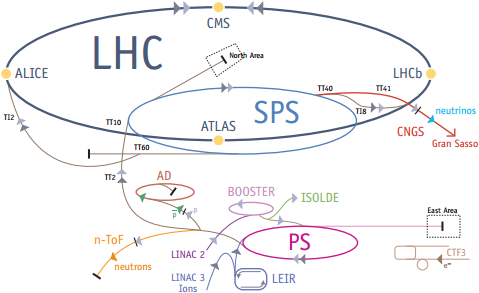
\includegraphics[width=300px]{lhcb/lhc.png}
\caption{\small The LHC Accelerator System}
\label{fig:lhc}
\end{figure}

The initial linear accelerator (LINAC2) accelerates protons to 50 MeV and 
feeds them through the Proton Synchrotron Booster (BOOSTER), which
accelerates them to 26 GeV. Finally, protons are injected into the LHC
complex at an energy of 450 GeV.

The four main LHC experiments situated at the beam crossing points shown in
figure~\ref{fig:lhc}: \atlas, \alice, \cms, \lhcb. \alice dedicated to heavy
ion physics. \atlas and \cms are general purpose detectors, which primary goal is
to discover new particles. More details on the \lhcb experiment, which collected the 
data set used in this thesis, are given in the next section.

The new particles are expected to have large masses and their production
processes have small cross sections, so the LHC machine is designed with both
a center-of-mass energy and a luminosity as large as possible.

The operation of the \lhc can be shown as follows: bunches of protons move in
opposite direction and are kept in orbit around the 27\km circumference of the accelerator by
the magnetic field generated by superconducting dipoles. A temperature of 2\degk is preserved
for magnets' coils to generate a maximum magnetic field of 8\tesla. This field
allows to produce the design center-of-mass energy of $\sqs=14\tev$.
Finally the bunches are designed to collide with a frequency of 40\mhz at the
interaction points to achieve a design luminosity of $10^{34}\cm^{-2}s^{-1}$.

The main LHC design parameters are shown in Table~\ref{tab:lhc}.

\begin{table}[t]
\caption{\small The main LHC design parameters}
\centering
\begin{tabular}{rr}
Circumference & 27\km\\
Center-of-mass energy & 14\tev\\
Injection energy & 450\gev\\
Field at 2 $\times$ 450\gev & 0.535\tesla\\
Field at 2 $\times$ 7\tev & 8\tesla\\
Helium temperature & 2\degk\\
Luminosity & $10^{34}\cm^{-2}s^{-1}$\\
Bunch spacing & 25\ns\\
Luminosity lifetime & 10\hr\\
Time between 2 fills & 7\hr\\
\end{tabular}
\label{tab:lhc}
\end{table}

\section{The LHCb experiment}
\label{ch_lhcb:lhcb}

The \lhcb detector is a forward single-arm spectrometer with forward angular
momentum coverage from 10 mrad to 300 mrad in the bending plane and 10 mrad to
250 mrad in the non-bending plane. These planes are defined by the 
direction of the field generated by a dipole magnet. The choice of the unique LHCb geometry is
justified by the fact, that b-hadrons are predominantly produced in a narrow
angular cone in the same forward and backward directions.

\begin{figure}[tb]
\begin{center}
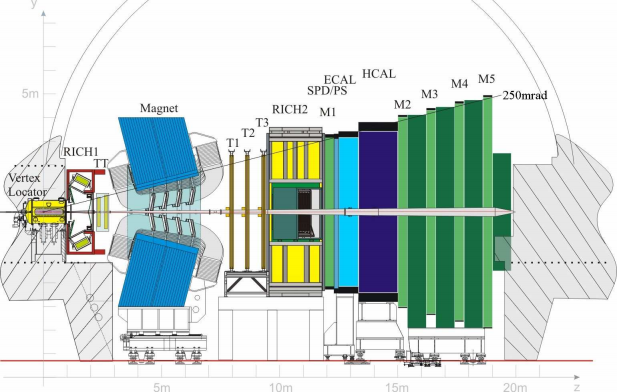
\includegraphics[width=300px]{lhcb/lhcb.png}
\end{center}
\caption{\small Schematic layout of the LHCb detector~\cite{Alves:2008zz}. 
The interaction point where the protons collide is on the left of the figure, 
and sub-detectors are labeled.}
\label{fig:lhcb}
\end{figure}

LHCb allows the full reconstruction of exclusive decays of the b- and c-hadrons
in a variety of leptonic, semi-leptonic and purely hadronic final states. 
In order to achieve this goal and extract the physics of interest, 
specialized sub-detectors involved within the LHCb detector to perform the 
following major tasks:

\begin{itemize}

\item {\bf Precision vertexing}: a sufficient separation between primary and 
secondary vertices is required to efficiently select b-hadron candidates 
and allow time dependent analyses to be performed. Such measurements are 
performed by the VErtex LOcator (\velo).

\item {\bf Invariant mass determination}: a very good invariant mass
resolution is required in order to maximize the significance of signal with
respect to background. Therefore, precision energy and momentum estimates of
reconstructed tracks must be performed. This is achieved by \lhcb's tracking
and calorimetry systems.

\item {\bf Particle identification}: hadronic decays of b- and c-hadrons, 
having identical topology but different flavour content in the final state, 
may peak at a common invariant mass; additional information is required to 
distinguish them from one another. 
Discrimination between charged hadrons (particularly pions and kaons) is 
achieved with a high performance Ring Imaging CHerenkov (RICH) system, 
whilst electrons, photons and muons are identified via the 
Calorimeter and Muon systems, respectively.

\item {\bf Flexible and robust trigger and data acquisition}: this is required 
in order to cope with rapid changes in running conditions and physics 
interests. A dedicated multi-stage trigger, capable of selecting many different 
final states in an hadronic environment, reduces the data rate from the initial 
40\mhz of ``visible interactions'' to 5\khz which is suitable for 
offline storage and analysis.
\end{itemize}

Figure~\ref{fig:lhcb} presents the layout of the detector sub-systems 
within the LHCb detector. More details on each sub-detector will be given in 
the next sections.

\section{Tracking system}

The tracking system is an important part of the LHCb detector that collects such
information about charged particles as vertexing (determining the distance
between the production and the decay vertex of the b hadrons) and
momentum reconstruction. These two together are used for reconstruction of the mass,
the angular and the proper time resolution, that are important for signal
selection and background suppression during the offline analysis of
$\chi_b \rightarrow \Upsilon \gamma$. Besides this, momentum and decay distance
information about momentum and decay distance are used in the trigger.

The LHCb tracking system is composed of a dipole magnet, the VELO and four 
planar tracking systems: the Tracker Turicensis (TT) upstream of the dipole 
magnet and three tracking stations T1, T2 and T3 downstream of the magnet. 
The latter three stations cover the entire geometrical acceptance of the 
spectrometer. To achieve the excellent tracking performance and also due to 
track multiplicity considerations, these three stations are composed of two 
distinct parts called the Inner Tracker (IT) and Outer Tracker (OT). 
The VELO, TT and IT use silicon strip technology while straw tubes are 
employed in the OT.\@ In fact, the TT and IT share a common technology, 
and they are called collectively the Silicon Tracker (ST). They have a very similar layout
sharing the same silicon microstrip technology with a strip pitch
of $200\mum$. Each of the four ST stations is composed of four detector 
layers with the strip directions arranged in a so called x-u-v-x layout: 
the first and fourth layers have vertical readout strips, while second (u) 
and third (v) layers have the strips rotated by a stereo angle of $+5^\circ$ 
and $-5^\circ$ respectively. This layout is designed to have the best hit
resolution in the x direction (in the bending plane), without losing the 
stereo measurement of the tracks.

\subsection{Vertex Locator}

To provide precise measurements of track coordinates close to the interaction 
region, the Vertex Locator (VELO), consisting of a series of silicon modules, 
is arranged along the beam direction. It is used to identify the detached 
secondary vertices typical for b-hadron decays and makes it possible to meet 
the requirement to reconstruct B decays
with a proper time resolution good enough to resolve the fast time-dependent
oscillations or CP asymmetries.

To provide accurate measurements of the position of the vertices, the silicon
modules of the VELO are placed closed to the beam axis, namely at 8\mm.
In order to detect the majority of the tracks originating
from the beam spot ($\sigma$ = 5.3\cm along the beam direction), 
the detector is designed such that
tracks emerging up to $z = 10.6\cm$ downstream from the nominal interaction
point cross at least 3 VELO stations, for a polar angular window between 15
and 300\mrad, as shown in Figure~\ref{fig:velooverview}.

\begin{figure}[tb]
\begin{center}
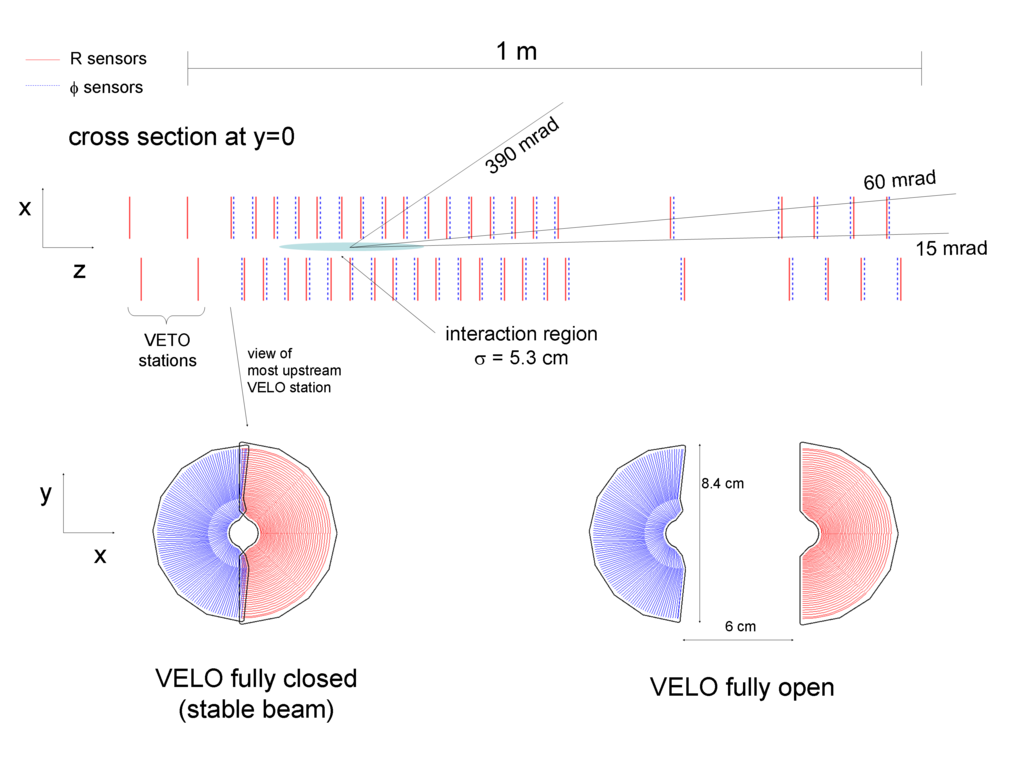
\includegraphics[width=300px]{lhcb/velooverview.png}
\end{center}
\caption{\small The setup of the VELO silicon modules along the beam direction.
The left two pairs form the pile-up system. Indicated are the average crossing
angle for minimum bias events (60\mrad), and the minimal (15\mrad) and
maximal (390\mrad) angle for which at least 3 VELO stations are crossed.
390\mrad is the opening angle of a circle that encloses a rectangular opening
angle of 250 $\times$ 300\mrad}
\label{fig:velooverview}
\end{figure}

To enable fast reconstruction of tracks and vertices in the \lhcb trigger,
a cylindrical geometry with silicon strips measuring $r\phi$ coordinates is
chosen for the modules.

The strips of the r sensor are concentric semi-circles, the $\phi$ sensors 
measure a coordinate almost orthogonal to the r-sensor. The geometry is shown in
Figure~\ref{fig:velomodule}. A 2D reconstruction in the r-z plane alone allows to
detect tracks originating from close to the beam line in the high-level trigger.
These measurements are used to compute the impact parameter of tracks with
respect to the production vertex, which is used in the trigger to discriminate 
between signal and background. The level-0 trigger uses information from the
pile-up veto system, two stations located upstream, which make it possible to
reject events with multiple pp interactions in one beam crossing.

\begin{figure}[H]
  \setlength{\unitlength}{1mm}
  \centering
  \resizebox{\textwidth}{!}{
  \begin{picture}(150,80)
    \put(0,0){
        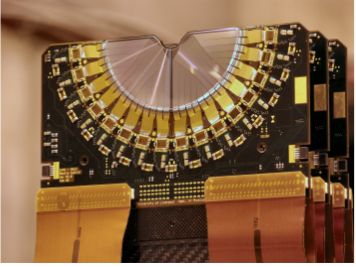
\includegraphics[width=.45\textwidth]{lhcb/velosensor}
    }
    \put(75,0){
        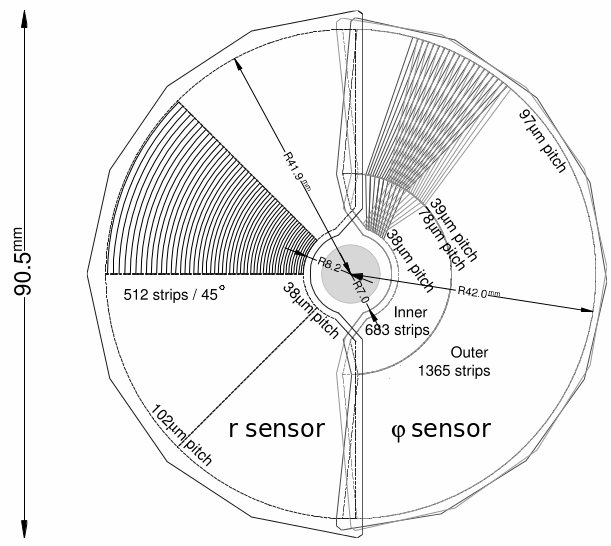
\includegraphics[width=.45\textwidth]{lhcb/velomodule}
    }
  \end{picture}
  }
\caption{The \velo r-sensors (left) and $\phi$-sensors (right).}
\label{fig:velomodule}
\end{figure}




The setup of the \velo is as follows. The half disc sensors are arranged in
pairs of r and $\phi$ sensors and are mounted back-to-back. The sensors are 300
$\mu m$ thick, radiation tolerant, n-implants in n-bulk technology. The
minimal pitch of both the r and the $\phi$ sensors is 32 $\mum$, linearly
increasing towards the outer radius at 41.9 mm. To reduce the strip occupancy
and pitch at the outer edge of the $\phi$-sensors, the $\phi$-sensor is divided
in two parts. The outer region starts at a radius of 17.25 mm and has
approximately twice the number of strips as the inner region. The strips in
both regions make a $5^\circ$ stereo angle with respect to the radial to
improve pattern recognition, and adjacent stations are placed with opposite
angles with respect to the radial. In order to fully cover the azimuthal angle
with respect to the beam axis, the two detector halves overlap, as is shown in
Figure~\ref{fig:velomodule}.

To minimize the amount of material traversed by particles 
before reaching the active detector layers, the detector is placed inside vacuum. 
To separate the primary beam vacuum from the secondary 
vessel vacuum and shield the detector
from RF pickup from the beam, the sensors are separated from the beam vacuum by
a thin aluminum foil. Both the sensors and this commonly named RF-foil are
contained inside a vacuum vessel. During beam injection the two halves of the
VELO are retracted 3\cm away from the nominal beam position. The RF-foil is
designed to minimize particle interactions.

\subsection{Magnet}

To provide a good momentum resolution, the \lhcb experiment utilizes a (dipole)
magnet (see Figure~\ref{fig:magnet}), which bends the tracks of charged
particles. The non-superconducting magnet consists of two saddle-shaped coils.
These are placed mirror symmetrically, such that the gap left open by the
magnet is slightly larger than the \lhcb acceptance, and the principal field
component is vertical throughout the detector acceptance.

\begin{figure}[tb]
\begin{center}
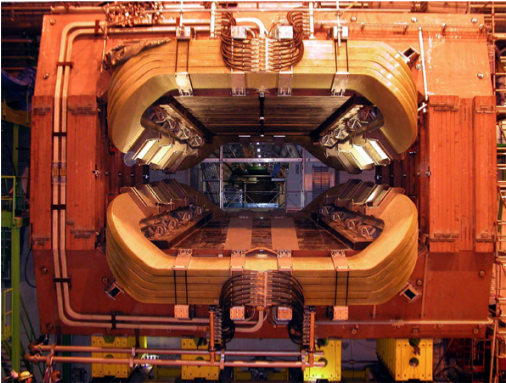
\includegraphics[width=300px]{lhcb/magnet}
\end{center}
\caption{\small The \lhcb dipole magnet. The proton-proton interaction
region lies behind the magnet.}
\label{fig:magnet}
\end{figure}


The quantity important for momentum resolution, and hence for the analysis of
channels such as $\chi_b \rightarrow \Upsilon \gamma$, is the integrated magnetic field
the magnet delivers. For tracks passing through the entire tracking system this
is
\cite{Alves:2008zz}:   

$$ \int Bdl = 4 Tm $$ making it possible to measure charged particles' momenta
up to 200\gev within 0.5\% uncertainty.

\subsection{Inner tracker}

\begin{figure}[tb]
\begin{center}
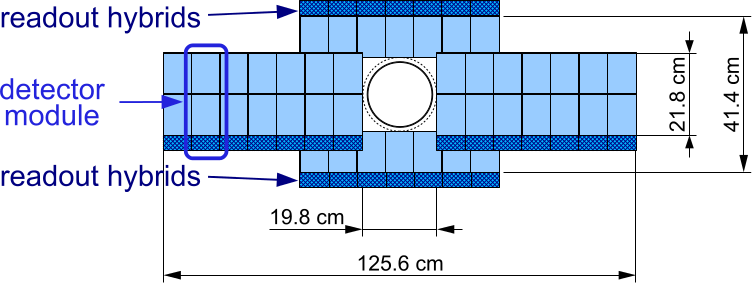
\includegraphics[width=300px]{lhcb/veloit}
\end{center}
\caption{\small Layout of the \intr.}
\label{fig:veloit}
\end{figure}

To perform accurate momentum estimates, important for mass, angular and proper
time resolutions in the reconstruction of the interesting physics channels, 
hit information downstream of the magnet is required, which is
provided by three tracking stations. Since the magnet bends particles in the
horizontal direction perpendicular to the beam pipe, the track density is
largest in an elliptically shaped region around the beam pipe. In order to have
similar occupancies over the plane, a detector with finer detector granularity
is required in this region. Therefore, the Inner Tracker (IT), 120\cm wide and
40 cm high, as shown in Figure~\ref{fig:veloit}, is located in the center of
the three tracking stations.



Due to the high track density near the beam pipe, silicon strip detectors are
used. The total active detector area covers 4.0 $m^2$, consisting of 129024
readout strips of either 11\cm or 22\cm in length. To improve track
reconstruction, the four detector layers are arranged in an x-u-v-x geometry,
in which the strips are vertical in the first and in the last layer, whereas
the other two (u, v) layers are rotated by stereo angles of $\pm5^\circ$,
providing the sensitivity in the vertical direction.

The pitch of the single-sided $p^+$-on-n strips is $198\mum$. In order to have
similar performance in terms of signal-to-noise, the thickness of the sensors
is $320\mum$ for the single-sensor ladders below and above the beam pipe, and
$410\mum$ for the double sensors at the sides of the beam pipe. The four
layers are housed in 4 boxes, which are placed such that they overlap. These
overlaps avoid gaps in the detector and, more importantly, make it possible to
perform alignment using reconstructed tracks.



\subsection{Outer tracker}

Similar to the \intr, the Outer Tracker (\ot) performs track measurements
downstream of the magnet, allowing to determine the momenta of charged
particles. The OT covers the outer region of the three tracking stations T1--T3.

Since the track density further away from the beam pipe is lower, straw tubes
are used. The total active area of one station is $5971\times4850\mm^2$, and
the \ot and the \intr together cover the full acceptance of the experiment. As is
the case for the \intr, these layers are also arranged in an x-u-v-x geometry, as
shown in Figure~\ref{fig:veloot}.

\begin{figure}[tb]
\begin{center}
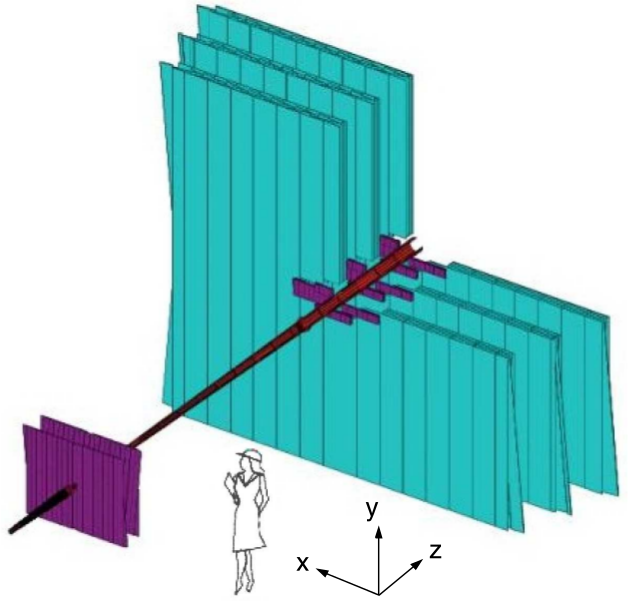
\includegraphics[width=300px]{lhcb/veloot}
\end{center}
\caption{\small Layout of the OT.}
\label{fig:veloot}
\end{figure}

The OT is designed as an array of individual, gas-tight straw-tube modules.
Each module contains two layers of drift-tubes with an inner diameter of
4.9\mm. The front-end (FE) electronics measures the drift time of the
ionization clusters produced by charged particles traversing the straw tubes,
digitizing it with respect to every bunch crossing. Given the bunch crossing
rate of 25\ns and the diameter of the tube, and in order to guarantee a fast
drift time (below 50\ns) and a sufficient drift-coordinate resolution
(200\mum), a mixture of Argon (70\%) and CO2 (30\%) is used as counting gas.

\subsection{Tracker Turicensis}

To improve the momentum estimate of charged particles, track measurements are
performed before these enter the magnet. Therefore, the Tracker Turicensis
(TT), a planar tracking station, is located between the VELO and the LHCb
dipole magnet. It is also used to perform the track measurements of long lived
neutral particles which decay after the VELO.\@ In addition, by using the weak
magnetic field inside the tracker, track information from the TT is used by the
High Level Trigger to confirm candidates between the VELO and the tracking
stations.

In order to cover the full acceptance of the experiment, the TT is constructed
150 cm wide and 130 cm high. It consists of four detector layers, with a total
active area of $8.4\m^2$, with 143360 readout channels, up to 38\cm in length.
To improve track reconstruction, the four detector layers are arranged in two
pairs that are separated by approximately 27\cm along the \lhcb beam axis. And
again, like the IT and the OT, the TT detection layers are in an x-u-v-x
arrangement.

\begin{figure}[tb]
\begin{center}
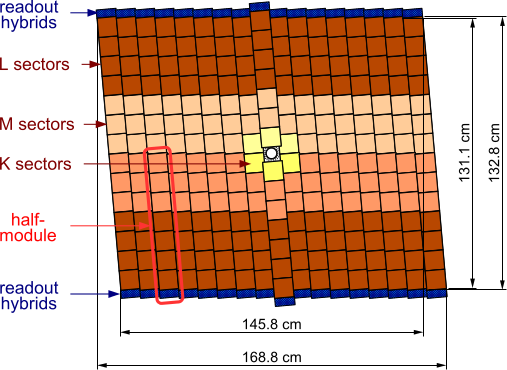
\includegraphics[width=300px]{lhcb/velott}
\end{center}
\caption{\small Layout of one of the stereo plane detector layers of the \ttracker}
\label{fig:velott}
\end{figure}


The layout of one of the detector layers is illustrated in
Figure~\ref{fig:velott}. Its basic building block is a half module that covers
half the height of the \lhcb acceptance. It consists of a row of seven silicon
sensors, named a ladder. The silicon sensors for the \ttracker are $500\mum$
thick, single sided $p^+$-on-n sensors, as for the IT.\@ They are
$9.64\cm\times9.44\cm$ long and carry 512 readout strips with a strip pitch of
$183\mum$.

\section{Particle identification}

Particle identification (PID) is a fundamental requirement for \lhcb. It is
essential for the goals of the experiment to separate pions from kaons in
selected B hadron decays.

\subsection{\rich system}

There are two \rich detectors in \lhcb. \richone is located before the magnet
(between the \velo and \ttracker) and are used for identification of low momentum
particles. RICH2 is located behind the magnet (between \ot and M1) and is
used for the identification of high momentum particles. The combination of both
detectors allows for kaon and pion separation in the momentum range $2 < p <
100 \gevc$.

\begin{figure}[tb]
\centering
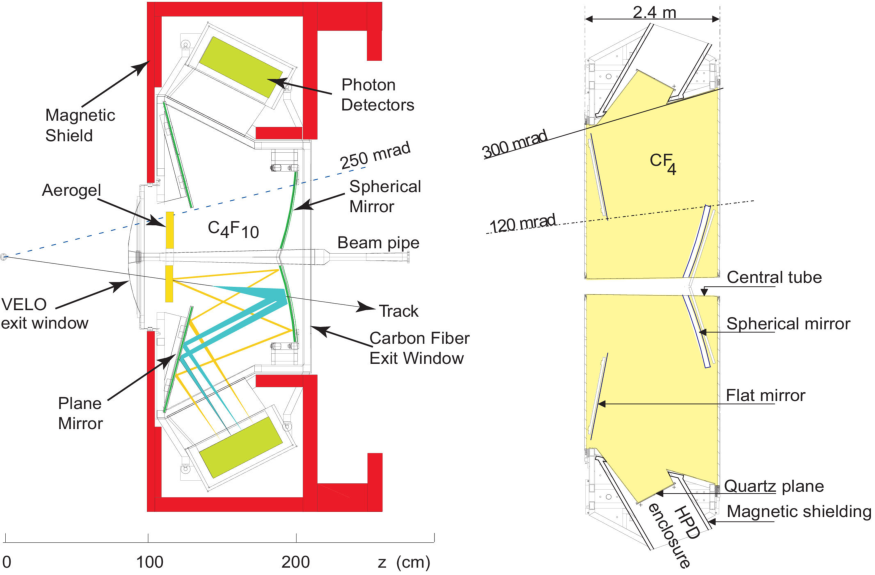
\includegraphics[width=.75\textwidth]{lhcb/rich}
\caption{\small Layout of the \richone(left) and \richtwo(right) detectors.}
\label{fig:rich}
\end{figure}

The RICH detectors measure the opening angle of the Cherenkov emission cone
produced by a charged particle that traverses the medium. The photon emission
is focused on the detector surface using a combination of spherical and flat
mirrors. The mirrors are tilted to allow the photo detectors to be positioned
outside the active area of the detector.

The Cherenkov emission angle $\theta$ is given by:
$$\cos\theta = \frac{1}{n\beta}$$
\noindent where n is the refractive index of the radiator medium and 
$\beta = v/c$ is the velocity of the particle. Given the momentum p of a
particle and the emission angle $\theta$, the particle mass and therefore the
type can be determined.

The \richone and \richtwo detectors have different effective momentum ranges,
which are determined by the corresponding radiator emission threshold velocity
$\beta_{thr} = 1/n$. The \richone detector uses a combination of aerogel and
$C_4F_{10}$ gas radiators and covers the low momentum range $1<p<60 \gevc$. The
\richtwo detector uses a $CF_4$ radiator and covers the high momentum range $15
< p < 100 \gevc$.

\subsection{Muon system}

The \lhcb muon system is designed for muon identification and tracking. It
provides information on the transverse energy of the muon to the first level
trigger (L0) and muon-ID for the second level trigger (HLT) and offline
analysis.

\begin{figure}[tb]
\begin{center}
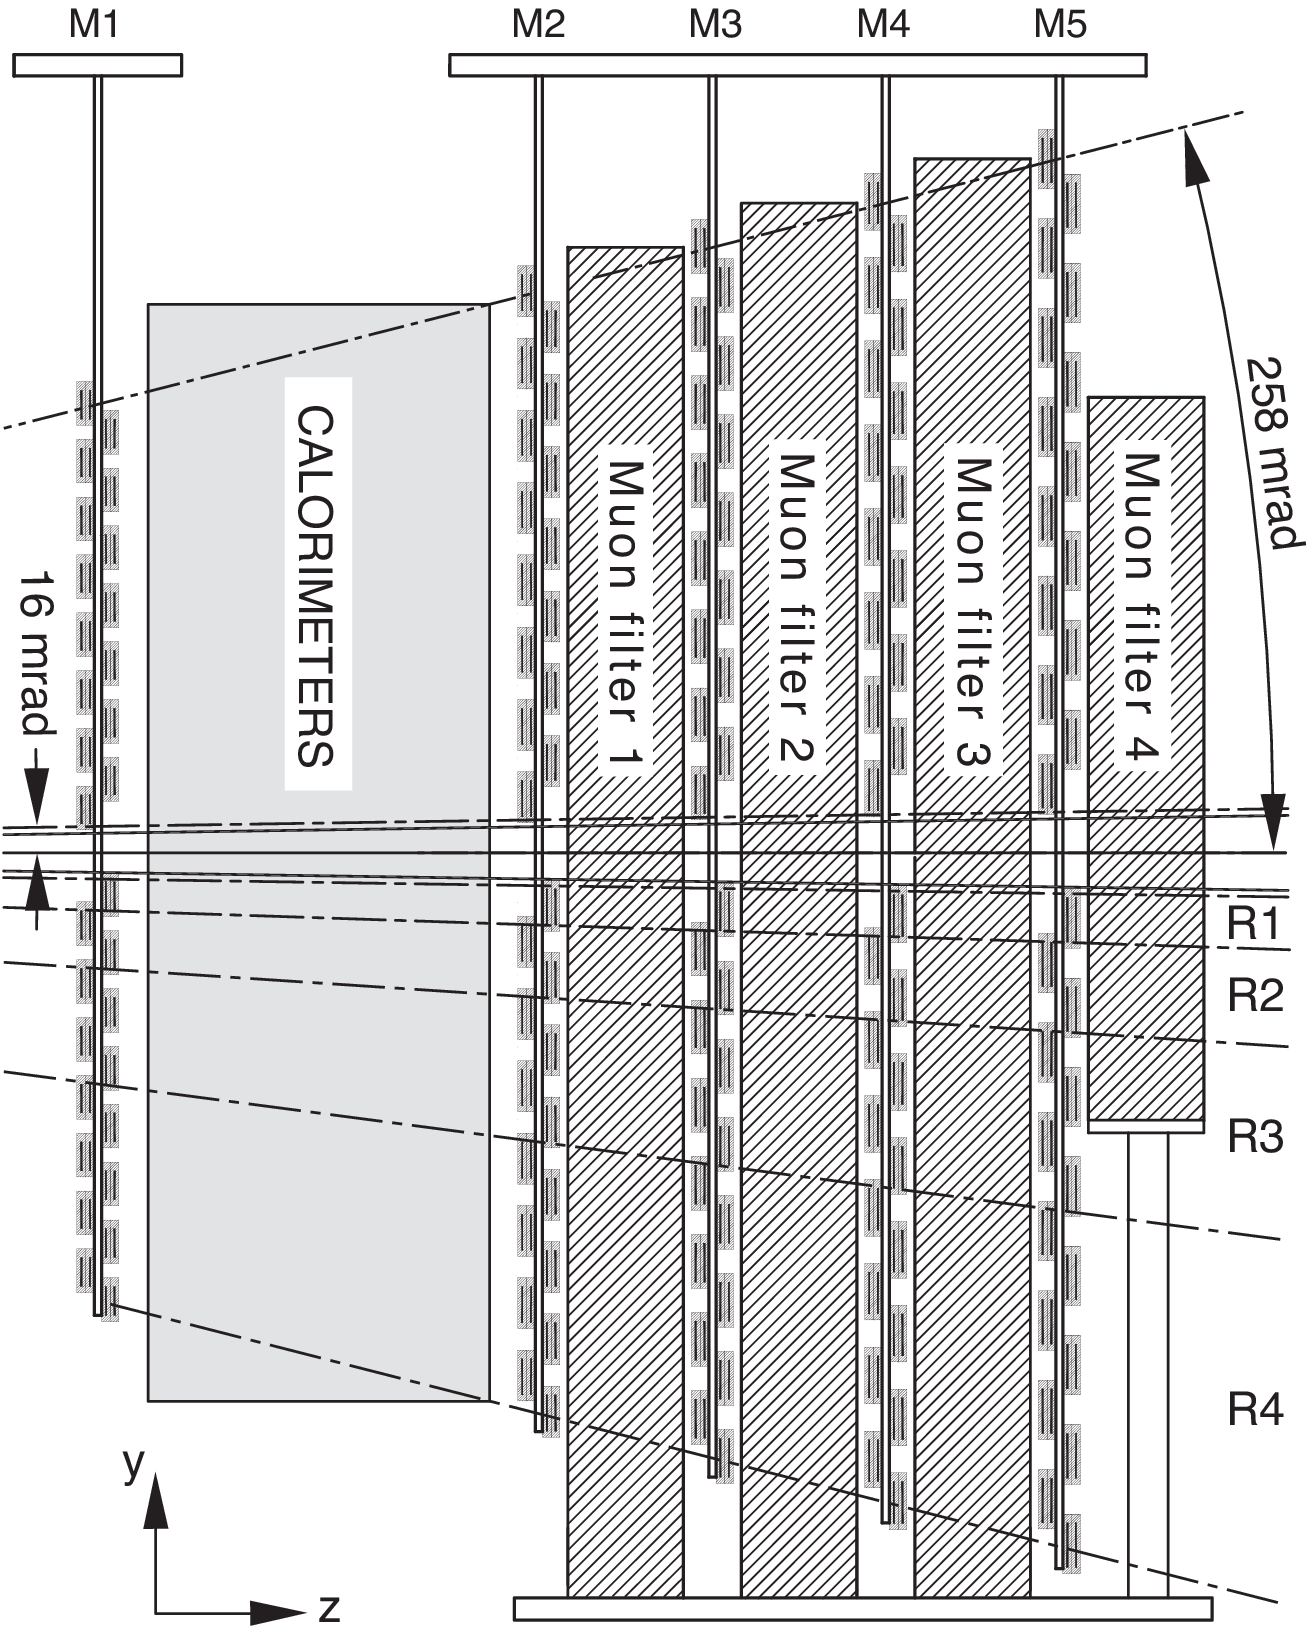
\includegraphics[width=.75\textwidth]{lhcb/muon}
\end{center}
\caption{\small Layout of the muon system.}
\label{fig:muon}
\end{figure}

The muon system is composed of five stations (M1--M5) placed along the
beam axis (Figure~\ref{fig:muon}). Stations M2 to M5 are placed downstream of the
calorimeters and are interleaved with iron absorbers. The M1 station is
located in front of the \spd/\presh and is used to improve the transverse momentum
estimate in the trigger. Each station is divided into four regions, R1 to R4,
with increasing distance from the beam axis. The granularity of each region is
made according to the particle flux, keeping the channel occupancy roughly
constant over the four detector regions. For more precise momentum measurement
the granularity is higher in the horizontal plane.
Muon chambers are the building blocks of the muon system. They are composed of 
two types of detectors: Multi Wire Proportional Chambers (MWPC), and triple GEM detectors. 
The latter are used in the inner region of M1, where the expected particle rate exceeds 
the safe MWPC ageing limit. Twelve GEMs are placed in the higher track density region, 
while the total system comprises 1392 chambers of various sizes. The MWPCs are 
subdivided in four tungsten gaps 5$mm$ thick and filled with a gas mixture of 
$Ar$ (50\%), $CO_2$ (40\%) and $CF_4$ (10\%). Inside the gaps, wires with 
a diameter of 30$\mu m$ are placed at a distance of 2$mm$ from each other. 

\subsection{Calorimeter system}

The calorimeter system is designed to measure the energy and position of
hadrons, electrons and photons. This information is used in the first level
trigger (L0) as well as in the offline analysis.

The calorimeter system is located between the RICH2 and muon detectors and
consists of a scintillator pad detector (SPD), a pre-shower detector (\presh), an
electromagnetic calorimeter (\ecal) and a hadronic calorimeter (\hcal). The \spd
and PS are located in front of the \ecal and provide information on the
evolution of the electromagnetic shower. The \ecal serves to measure the energy
of electrons and photons, whereas the \hcal measures the energy of hadrons.

When a particle hits the calorimeter, it produces a cascade of secondary
particles. These secondary particles excite the scintillator material, which in
turn emits the scintillation light. The light is transmitted through
wavelength-shifting fibers to the photomultiplier tubes. The total amount of
light collected by photomultipliers is proportional to the energy of the
incident particle.

The SPD and PS consist of scintillator pads, separated by a 15\mm thick lead
converter. The SPD is used for identification of charged particles before the
start of the shower. The lead converter initiates the shower that subsequently
is detected by the PS.\@ The SPD allows to separate electrons from photons,
whereas the PS is used for separation of electrons and photons from hadrons.

The ECAL consists of lead-scintillator modules and covers the acceptance of
$25<\theta_x< 300\mrad$ and $25 < \theta_y < 250\mrad$ in the horizontal and
vertical planes, respectively. Each module is 42\mm thick and consists of
alternating layers of 4\mm scintillator material and 2\mm lead absorber. The
modules vary in size from $4\times4\cm^2$ in the inner part of the detector, to
$6\times6\cm^2$ in the middle and $12\times12\cm^2$ in the outer part of the
detector. The energy resolution of \ecal for electrons and photons is: 

\begin{equation}
\left(\frac{\sigma_{E}}{E}\right)_{\ecal} = \frac{10\%}{\sqrt{E\left[\gev\right]}} \oplus 1\%
\label{eqn:ecal}
\end{equation}

The HCAL is located behind the \ecal. The modules of the HCAL have dimensions of
$13\times13\cm^2$ and $26\times26\cm^2$ in the inner and outer part of the
detector, respectively, and consist of alternating layers of 1\cm thick iron
and scintillators. The energy resolution of \hcal for hadrons is:

\begin{equation}
\left(\frac{\sigma_{E}}{E}\right)_{\hcal} = \frac{80\%}{\sqrt{E\left[\gev\right]}} \oplus 10\%
\label{eqn:ecal}
\end{equation}

\section{Trigger}

The \lhcb trigger system is used for the selection and storage of events for
LHCb physics studies. The general layout of the trigger is shown in Fig. 2.12.
The first level trigger Level-0 (L0) is implemented in hardware. The L0 trigger
decision is based on the information of the calorimeter and muon systems. Both
systems provide information on the multiplicity, and transverse energy \et or
transverse momentum \pt of individual particles. The High Level Trigger (HLT)
is the second level trigger of \lhcb. The HLT is a software trigger that runs on
about 15000 processors of the Event Filter Farm. The HLT, with its two stages
HLT1 and HLT2, reduces the 1\mhz L0 rate to about 5\khz which is permanently 
stored. 

HLT1 reduces the rate from 1\mhz to 50\khz. HLT1 performs the reconstruction
of particles in the \velo and determines the location of primary vertexes and
impact parameters (IP) of the particles. The events are selected based on the
presence of particles which pass the requirements on the minimum track quality,
IP, momentum, and transverse momentum. These selections are based on the decay
kinematics of charm and beauty hadrons, such as:

\begin{itemize}
\item high average momentum and transverse momentum of charm and beauty
hadrons, and consequently their decay products;
\item the decay vertex is well displaced from the collision (primary) vertex, and
consequently the reconstructed final state particles on average do not point
to the primary vertex.
\end{itemize}

HLT2 reduces the rate from 50\khz to 5\khz and is mainly based on inclusive
trigger lines that cover most of the B decays with displaced vertexes. In
addition, HLT2 contains trigger lines based on the presence of muons and lines
aiming at selecting exclusive B decays. HLT2 uses similar requirements on the
particles as HLT1, in addition to which the requirements on distance between
primary and secondary vertexes, vertex quality, mass and lifetime are used.
\Cref{fig:hlt} shows HLT schematic overview.

\begin{figure}[H]
  \setlength{\unitlength}{1mm}
  \centering
  \resizebox{\textwidth}{!}{
  \begin{picture}(170,55)
      \newsavebox{\hltbox}
      \savebox{\hltbox}(50,55)[bl]{
        \multiput(0,0)(30,0){2}{\line(0,1){55}}
        \multiput(0,0)(0,55){2}{\line(1,0){30}}
        \put(30,27){\vector(1,0){20}}
      }
      \put(0,0){\usebox{\hltbox}}
      \put(5,50){\bf L0}
      \put(5,35){$p_T^{\mu}$}
      \put(5,29){$p_T^{\mu_1}$, $p_T^{\mu_2}$}
      \put(5,23){$E_T$ - hadron}
      \put(5,16){$E_T$ - electron}
      \put(5,10){$E_T$ - $\gamma$, $\pi$}
      \put(32,29){$1.1\mhz$}

      \put(50,0){\usebox{\hltbox}}
      \put(55,50){\bf HLT1}
      \put(55,35){technical}
      \put(55,29){single $e$}
      \put(55,23){1 track all}
      \put(55,16){1 track $\mu$}
      \put(55,10){$\mu$, $\mumu$}
      \put(82,29){$50\khz$}


      \put(100,0){\usebox{\hltbox}}
      \put(105,50){\bf HLT2}
      \put(105,40){technical}
      \put(105,34){exotics}
      \put(105,28){EW}
      \put(105,22){B2HH}
      \put(105,16){radiative}
      \put(105,10){charm}
      \put(105,4){\mumu}
      \put(132,29){$5\khz$}
      \put(152,27){\bf Storage}
  
  \end{picture}
  }
\caption{Schematic overview of the LHCb trigger.}
\label{fig:hlt}
\end{figure}


\section{LHCb 2010--2012 operation}

\lhcb operated at center-of-mass energies of \sqs=7\tev in 2010-2011 and 
\sqs=8\tev in 2012. Figure~\ref{fig:lumi} shows the integrated luminosity
delivered and recorded by LHCb in these data-taking periods. In 2011 and 2012,
the operation conditions and luminosity were relatively stable and the total
recorded luminosity amounts to 1.107\invfb and 2.082\invfb in 2011 and 2012
respectively.

The data used in the analysis of $\chi_b$ production presented in this thesis
correspond to the full datasets collected in 2011 and 2012. 

\begin{figure}[tb]
\begin{center}
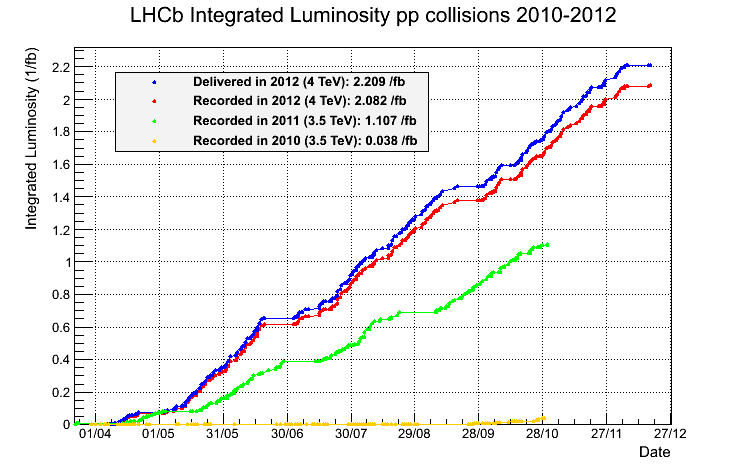
\includegraphics[width=.75\textwidth]{lhcb/lumi}
\end{center}
\caption{\small \lhcb integrated luminosity pp collisions 2010--2012.}
\label{fig:lumi}
\end{figure}

% \subsection{Software}
% \subsubsection{Core software}
% \subsubsection{Online software}
% \subsubsection{Grid infrastructure}

% \chapter{Performance profiling}
% \section{Introduction}
% \section{Profiling techniques}
% \subsection{Hardware counters}
% \subsection{Instrumenting the code}
% \section{Tools}
% \subsection{Valgrind}
% \subsection{Gperftools}
% \subsection{Intel VTune Amplifier}
% \subsection{Comparison}


\chapter{LHCb software performance profiling}
\chaptermark{Performance profiling}
\section{Introduction}

In \lhcb, as in all High Energy Physics (HEP) experiments, complex software is
used to process the data recorded by the detectors. Performance is an essential
characteristic of this software, especially when dealing with HLT: its role is
to filter events coming from the hardware based trigger in order to identify
those with interesting physics, and to write them to disk in real-time. The
number of events processed per second (event rate) is therefore one of the
crucial characteristics of the HLT, as it has to keep up with the data rate
delivered by the hardware triggers ($10^6$ events per second) in order to avoid
data loss. To reach such high throughput, the processing is performed on many
nodes in parallel by highly optimized algorithms. In order to optimize the
algorithms, and to keep track of the evolution of the event rate when changes
are applied to the HLT, it is necessary to measure the overall performance of
the code but also to understand which algorithms are costly in term of Central
Processing Unit (CPU) and computer memory.

In this chapter our focus is on the analysis of frequency and duration of
function calls in algorithms. This type of analysis is commonly named CPU
profiling. Profiling helps to identify parts of the code that take a long time
to execute. In performance analysis, those places often are referenced as
hotspots. Obviously,  hotspots affect the event rate of event processing
software. So, one of the main goals of profiling HEP software is to point out
to application developers the places in the code that need to be tuned to
increase the event rate.

The first study on CPU profiling at \lhcb was carried out by Daniele Francesco
Kruse and Karol Kruzelecki in their work ``Modular Software Performance
Monitoring''~\cite{modular}. They conclude that instead of profiling the
application as a whole it would be better to divide it into modules and profile
those modules separately. In general terms, a module can be defined as an
application's structural component that is used to group logically related
functions.  Grouping performance results by module allows a better insight into
where the performance issues are coming from. Since each module is under the
responsibility of a specific developer, the provided reports can be delivered
to the right person. For example, in the \gaudi~\cite{Barrand:2001ny} core
framework at LHCb each algorithm used for event processing is such a module
which can be profiled independently. More details on \gaudi will be given in
Section~\ref{sec:gaudi}.

This design principle was first implemented in a set of profiling tools based
on perfmon2~\cite{perfmon2} library. These tools have several drawbacks. First,
the produced analysis reports  used the  hardware event counters metrics. Only
developers with a good knowledge of the hardware  architecture could read and
interpret those reports. Since the major part of developers in HEP are
physicists, the number of users of those tools are very low. Second, since the
current tools do not use the counters multiplexing feature of perfmon2 library,
the target program should be run several times to collect all required hardware
counters. As a result, the profiling time is significantly increasing.

To fill some of the the gaps of the previous tools the Gaudi Intel
Profiling Auditor was created. This profiling tool uses the same module principle that was
described in~\cite{modular}, but is based on \iamp~\cite{vtune}.
\amp is the newer performance profiling tool, that provides better
functionality than perfmon2 library.

In the next section \iamp is briefly reviewed. Then it is discussed how the Gaudi
Intel Profiling Auditor can integrate \amp to the \gaudi framework, and examples 
of using those tools to profile \lhcb's HLT are shown. 

\section[VTune Amplifier]{\iamp}
This section gives an overview of \iamp profiling tool and
describes its basic features and analysis reports.

\subsection{Overview}
\iamp is a commercial application for software performance analysis that is
available for both Linux and Windows operating systems. \amp belongs to the
runtime instrumentation class of profiling tools. This means that the code is
instrumented before execution and the program is fully supervised by the tool.
A target application can be profiled without any modification of the codebase.

\iamp has  various kinds of code analysis including hotspot analysis,
concurrency analysis, locks and waits analysis. In Profiling Auditor a
hotspot analysis based on the user-mode sampling feature of \amp is used.
User-mode sampling allows to profile a program by exploring a call stack of a
running program and produce one simple metric --- the amount of time spent in the
function.

The amount of time spent in a function (CPU time) is calculated by interrupting
a process and collecting samples of call stacks from all active threads. The CPU
time value is calculated by counting the number of  a function's appearances at
the top of a call stack. This means that stack sampling is a statistical method
and does not provide a 100\% accurate measurement. However, for a large number
of samples the sampling error does not have a serious impact on the accuracy of
analysis. More details about sampling accuracy will be provided
in~\Cref{sec:accuracy}.

\amp also supports the hardware event-based sampling and provides advanced
metrics based on event counters inside a processor. Reports that use those
metrics require  knowledge of hardware architecture, unlike the user-mode
sampling reports that can be understood by any application developers.
Furthermore, while the user-mode sampling can be performed on any 32 and 64-bit
x86 based machine, the hardware event-based sampling is targeted only for a
specific \intel microarchitecture and requires a special driver to be installed
on the operating system. The advantage of the hardware event-based sampling is 
that it can be used for fine tuning of algorithms in places where  the user-
mode sampling could not point out the reasons for the hotspot.

The goal of our profiling tool is to provide analysis reports to a wider
audience of software developers and, therefore, for implementation we chose the
user-mode sampling method over hardware-mode sampling.

\subsection{Sampling interval}

The sampling interval is an important parameter of the user-mode sampling
method. It can impact on results accuracy and on total profiling time. \intel
recommends to use a 10 ms interval. Using this value the average overhead of
the sampling is about 5\% in the most applications. The minimum sampling
interval value depends on the operating system. For example, a 10 ms interval
is the minimum value for the old Linux kernel 2.4, whereas 1 ms is the minimum
value for the modern Linux $\ge$ 2.6 kernels.

To determine an appropriate sampling interval, one should consider the duration of the
collection, the speed of your processors, and the amount of software activity.
For example, if the duration of sampling time is more than 10 minutes, consider
increasing the sampling interval to 50 milliseconds. This reduces the number of
interrupts and the number of samples collected and written to disk. The smaller
the sampling interval, the larger the number of samples.

\subsection{Tools}

\amp has two major interfaces --- a command-line tool {\it amplxe-cl} and a
Graphical User Interface tool {\it amplxe-gui}. {\it Amplxe-gui} generally
plays a role of analysis results presenter, but can also be used as a wrapper
to the  command-line tool. {\it Amplxe-cl} is used to execute the profiling
supervisor with appropriate parameters.  The second important function of {\it
amplxe-cl} is to export CPU usage reports to CSV text format. This feature
allows to use collected data not only inside \amp, but also in external user
applications.

\subsection{Profiling reports}

In this section we review essential profiling reports that are available in
\amp. These reports can be obtained either from {\it amplxe-gui} or {\it
amplxe-cl tool}, but for short we present only GUI screenshots.

An ordered function's CPU time usage report is a basic report of almost at all
performance profilers (Figure~\ref{fig01}).

\begin{figure}[H]
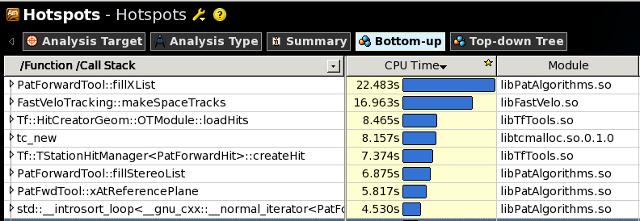
\includegraphics[width=\textwidth]{profiler/fig01.png}
\caption{Function's CPU Time report. The first column contains
function names. The second column is a CPU time usage and the last column
contains the names of the shared libraries where the functions are defined.}
\label{fig01}
\end{figure}

\amp provides many grouping options: 
\begin{figure}[H]
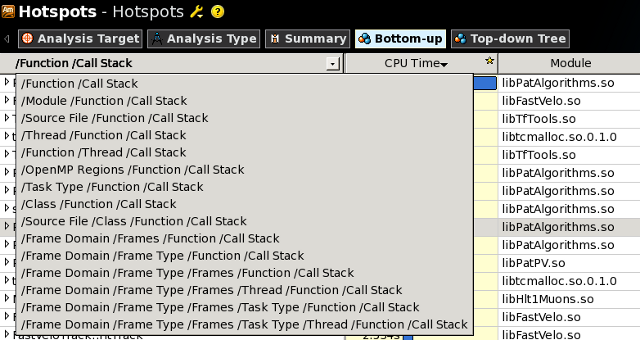
\includegraphics[width=\textwidth]{profiler/fig02.png}
\caption{Various grouping options.}
\label{fig02}
\end{figure}

Example of grouping by shared library:

\begin{figure}[H]
\begin{minipage}{\textwidth}
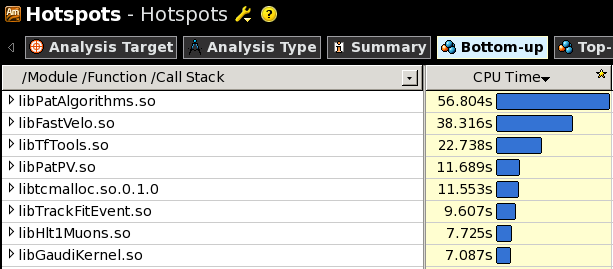
\includegraphics[width=\textwidth]{profiler/fig03.png}
\caption{\label{fig03}Shared libraries  CPU time report. First column contains
a name of shared library.}
\end{minipage}
\end{figure}


The striking feature of \amp is an ability to filter data based on a selection
in the timeline. This feature does not exists in other popular profilers:

\begin{figure}[H]
\begin{minipage}{\textwidth}
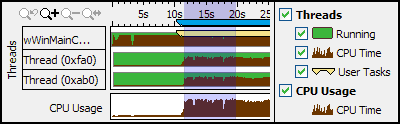
\includegraphics[]{profiler/fig04.png}
\caption{\label{fig04}Filter data on a selection in timeline.}
\end{minipage}
\end{figure}

CPU usage by code line can be created if a target application was compiled with
debug symbols:

\begin{figure}[H]
\begin{minipage}{\textwidth}
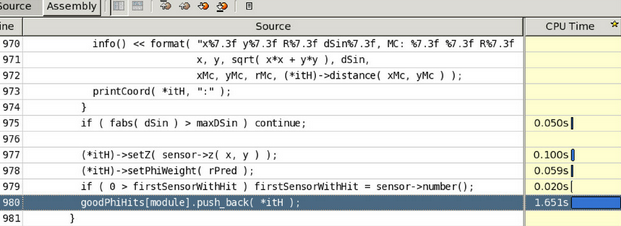
\includegraphics[width=\textwidth]{profiler/fig05.png}
\caption{\label{fig05}CPU time usage by code source line.}
\end{minipage}
\end{figure}

\subsection{Detecting code dependency}

Besides finding hotspots, another useful function of the profiling tool is to
reveal the code dependencies. Usually HEP applications have a lot of lines of
code and were developed by many people during a long period of time. Therefore,
determining relations between parts of code is very difficult. Since \amp  has
a top-down tree report of functions calls (Figure~\ref{fig06}.), we can
determine the code dependency in the application and see CPU usage in the call
chain.

\begin{figure}[H]
\begin{minipage}{\textwidth}
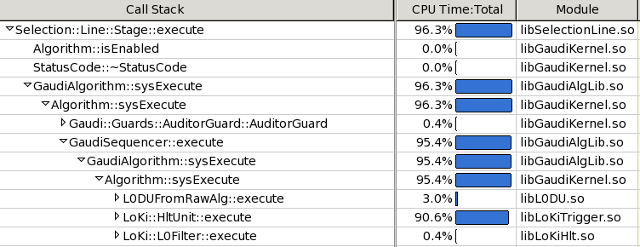
\includegraphics[width=\textwidth]{profiler/fig06.png}
\caption{\label{fig06}Top-down tree report.}
\end{minipage}
\end{figure}

\section[Profiling Auditor]{Gaudi Intel Profiling Auditor}

In the previous section we show that \iamp is a powerful performance profiling
tool. This section shows how this tool is used at \lhcb
for software optimization.

First, the \gaudi framework is described and then it is shown how the \gaudi Intel
Profiling Auditor can enhance \amp reports.

\subsection{Gaudi}
\label{sec:gaudi}
\gaudi is a C++ software framework used to build data processing
applications using a set of standard components. \gaudi is a core framework used
by several HEP experiments, in particular \lhcb and \atlas at \lhc. All 
event processing applications, including simulation, reconstruction, high-level
trigger and analysis are based on this framework. By design, the framework
decouples the objects  describing the data and those implementing the
algorithms. Due to this design,  developers can concentrate only on  physics
related tasks in algorithms and usually do not care about other parts of the
framework.

\begin{figure}[H]
\begin{minipage}{\textwidth}
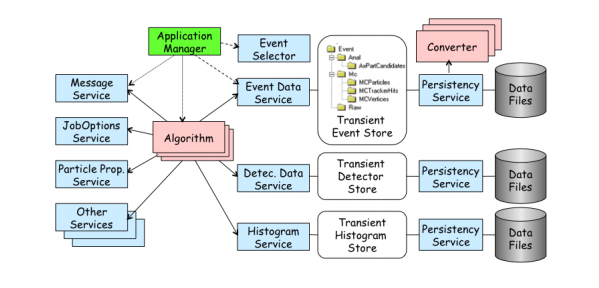
\includegraphics[width=\textwidth]{profiler/fig07.png}
\caption{\label{fig07}Gaudi Architecture (as described in
~\cite{Barrand:2001ny}). Applications are made by composing sequences of
Algorithms and adding specific Services and Tools.}
\end{minipage}
\end{figure}

The \gaudi framework is a highly customizable framework. Any component of the
system can be configured by user options.

\subsubsection{Gaudi Auditors}

The Application Manager is one of the major components of \gaudi. It takes care
of instantiating and calling algorithms. A supplement to this component  is the
Auditor Service that enable to add auditors to a \gaudi application. The auditor
is a set of user functions that are called on some workflow events in the
Manager. For example, we could add a custom action that is called when the
Manager wants to execute some algorithm or when an algorithm is finished. There
are many different events types and we can add as many auditors as needed. In
other frameworks and programming languages, this type of functions are often
referenced as callback functions.

In the following section we show how we can use an auditor to build a profiling
tool.

\subsection{Profiling Auditor}

\subsubsection{Objectives.}

A \gaudi application can be profiled by \amp  without any modifications of the
codebase.  This tool can collect any data about CPU consumption in code lines,
functions, classes, shared libraries, threads, but it has one disadvantage.
\amp knows nothing about \gaudi framework's algorithms. However, algorithms are
the central point of any framework application, since all major event processing
occurs there. In principle, a general task for framework users is just to write
algorithms that solve a problem and usually nothing more. So, if the profiler
could generate a report that can group function's CPU usage by algorithm, then
application developers could look to the profiling result from a new point of
view. This point of view can help to reveal previously invisible hotspots. In
order to provide such report the Gaudi Intel Profiler Auditor was developed.

\subsubsection{User API of \iamp.}

Each \gaudi algorithm has a name that is assigned to an algorithm at run-time.
\amp, in turn, is supplied with a C library that allows to import those names
to the target report. In order to use the library from user applications, the
public User API is provided in \amp. The API enables to control the data
collection process and set marks during the execution of the code. The
possibility to mark code regions at runtime is the crucial feature of our new
profiling tool, because the CPU usage in the region between algorithm's start and
finish points is exactly what is needed for the report that group functions by algorithm.
Event API is a part of the User API  that is in charge of marking.

\begin{description}
\item[\_itt\_event \_\_itt\_event\_create(const \_\_itt\_char \*name, int namelen );] \hfill \\
Create a user event type with the specified name. This API returns a handle to the user event type that should be 
passed into the following APIs as a parameter. The namelen parameter refers to the number of characters, 
not the number of bytes.

\item[int \_\_itt\_event\_start( \_\_itt\_event event );] \hfill \\
Call this API with an already created user event handle to register an instance of that event. This event appears 
in the Timeline panel display as a tick mark.

\item[int \_\_itt\_event\_end( \_\_itt\_event event );] \hfill \\
Call this API following a call to \_\_itt\_event\_start() to show the user event as a tick mark with a duration line 
from start to end. If this API is not called, the user event appears in the Timeline pane as a single tick mark.
\end{description}

\subsubsection{Implementation}

An auditor is a good component for implementing the required profiling tool. In
this case, we do not need to modify the algorithm's code and need only to write
two callback functions: at algorithm start and finish. In order to generate the
target report those functions need to call Event API functions of \amp.

An appropriate auditor was created and named \gaudi Intel Profiling Auditor. It
was deployed to the GaudiProfiling package of \gaudi framework as a shared
library. Below we show how this profiling tool marks regions and what reports
can be generated.

\gaudi has a special type of algorithms --- Sequence. Each instance of Sequence
can execute other algorithms or sequences. So, an application's event loop
could have not only a flat but also a tree structure. Moreover, the same
algorithm instance can occur in different sequences. Therefore, it was decided
that an algorithm's region between its start and finish should be marked by the
branch identifier. In this case, we get more detailed information about usage
of the algorithm in the application. A branch identifier is constructed from an
algorithm name and its parents in the sequence tree. For example, let's profile
an application that has the following sequence tree:
\begin{verbatim}
Hlt 
    HltDecisionSequence 
        Hlt1 
            Hlt1DiMuonHighMass
                Hlt1DiMuonHighMassFilterSequence
                    Hlt1DiMuonHighMassStreamer
                        FastVeloHlt
                        MuonRec
                        Velo2CandidatesDiMuonHighMass
                    GECLooseUnit
                        createITLiteClusters
                        createVeloLiteClusters
                Hlt1DiMuonHighMassL0DUFilterSequence
                    L0DUFromRaw
                    Hlt1DiMuonHighMassL0DUFilter
\end{verbatim}

In \amp the report that use information on marked regions can be obtained by
choosing the ``Task Type / Function / Call Stack'' grouping options as seen on
Figure~\ref{fig08}.

\begin{figure}[H]
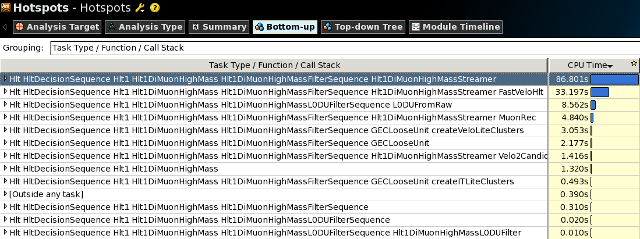
\includegraphics[width=\textwidth]{profiler/fig08.png}
\caption{Group and order CPU usage by branch identifier.}
\label{fig08}
\end{figure}

For example, the selected branch identifier {\it ``Hlt HltDecisionSequence Hlt1 Hlt1DiMuonHighMass Hlt1DiMuonHighMassFilterSequence Hlt1DiMuonHighMassStreamer''} in the report on Figure~\ref{fig08} is constructed from the names of algorithms that were executing 
when the \amp supervisor sampled a call stack. Each algorithm name in the branch is separated by the space. 

For each branch we could see a CPU usage by function (Figure~\ref{fig09}):

\begin{figure}[H]
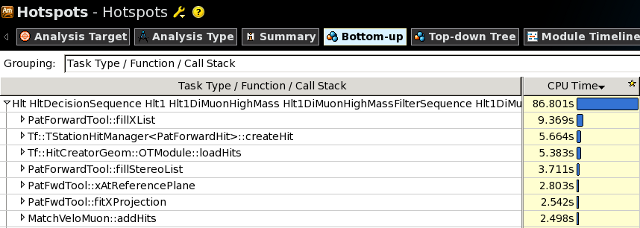
\includegraphics[width=\textwidth]{profiler/fig09.png}
\caption{Group and order CPU usage by branch identifier.}
\label{fig09}
\end{figure}

On Figure~\ref{fig09} we see the functions's CPU usage  in the algorithm {\it
Hlt1DiMuonHighMassStreamer\/} in the branch {\it ``Hlt~HltDecisionSequence~Hlt1
~Hlt1DiMuonHighMass~Hlt1DiMuonHighMassFilterSequence''}. As can be observed the
main goal was achieved --- we get the report that groups function CPU usage by
algorithm. So, the next step is only to interpret profiling results by
application developers and, if needed, to tune algorithms.

In addition to reports on algorithms, options were added in the \gaudi Intel Profiling 
Auditor, that allow to skip unimportant regions of the code during
profiling. Information about functions in those regions is not collected and,
as a result, we get clearer reports and a decrease of total profiling time. For
example, usually time critical processes happen in the event loop. Thus,
initialization and finalization phases are not interesting for developers. Due
to this, the auditor has options that trigger the start of  profiling on the
first event in the event loop and stop it after the last event.


\section{HLT Profiling Examples}

In the previous section we demonstrated how \gaudi Intel Profiler Auditor can
assist  in profiling \gaudi applications. The original motivation for creating
this auditor was a profiling of HLT applications of the \lhcb experiment. As 
stated in the introduction, trigger programs are most sensitive to the event
processing time. Therefore, a performance profiling is an essential tool for the 
developers of trigger applications. In this section we show three
examples of using \amp and \gaudi Intel Profiling Auditor to profile \moore, 
the \gaudi based HLT application at \lhcb.

\subsection{Memory Allocation Functions}

In the first example we profile a \moore program twice. The first time a program
was executed with the standard memory allocation function {\it operator new\/}
from {\it libstdc++\/} library:

\begin{figure}[H]
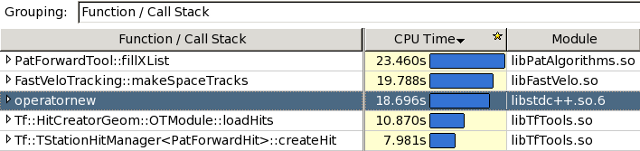
\includegraphics[width=\textwidth]{profiler/fig10.png}
\caption{Hotspot functions in the \moore application with the
standard memory allocation function.}
\label{fig10}
\end{figure}

\noindent and the second time it was executed with the memory allocation function {\it
tc\_new} from tcmalloc library~\cite{perftools}:

\begin{figure}[H]
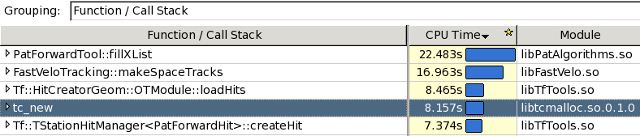
\includegraphics[width=\textwidth]{profiler/fig11.png}
\caption{Hotspot function in the \moore application with the memory allocation functions from tcmalloc 
library.}
\label{fig11}
\end{figure}

The figures indicates that {\it tc\_new} function is twice faster than {\it
operator new}. Moreover, a total application time reduction of 5\% was
observed if we replace standard allocation functions with function from
tcmalloc library.

\subsection{Measuring Profiling Accuracy}
\label{sec:accuracy}
To check the CPU time measurement accuracy we compared the results obtained by
the \gaudi Intel Profiler Auditor and by the \gaudi Timer Auditor. The Timer
Auditor proceeds in the same way as the Profiler Auditor --- it calculates the
difference between the algorithm's finish time and the time at the start of the
algorithm. Unlike the \gaudi Intel Profiler Auditor, the Timer Auditor
calculates the exact time spent in the algorithm. So, we can assume a CPU time
observed by the Timer Auditor as a reference value. The limitation of the Timer
is that it creates reports only for algorithms times  and could not provide
results for a low level of granularity (for functions or code instructions).
Therefore, only the algorithm's CPU times were compared.

Since the VTune Amplifier XE instruments the code before execution, the
absolute CPU time measured by the Profiler can differ from the time measured by
the Timer auditor.  But the time distribution of all algorithms should stay the
same in both auditors.  So, for the test we took a real HLT application and run
it twice, by using the Timer auditor the first time and the \gaudi Timer Auditor 
the second time. We then selected five hotspot algorithms and
calculated their time distribution relative to the top hotspot algorithm. The
process was repeated three times with different numbers of events: 10
(Table~\ref{tab:tevents10}), 100 (Table~\ref{tab:tevents100}) and 1000 events
(Table~\ref{tab:tevents1000}):

\begin{table}[H]
\caption{10 events}
\label{tab:tevents10}
\begin{center}
\begin{tabular}{rrrr}\toprule
Algorithm name & Timer (\%) & Profiler (\%) & \bf{Difference} \\
\midrule
L0Muon & 100 & 100 & -\\
Hlt1TrackAllL0Unit & 63.71 & 63.571 & \bf{0.139}\\
FastVeloHlt & 33.065 & 7.143 & \bf{25.922}\\
L0Calo & 8.065 & 0 & \bf{8.065}\\
HltPVsPV3D & 4.032 & 0 & \bf{4.032}\\
\bottomrule
\end{tabular}
\end{center}
\end{table}

\begin{table}[H]
\caption{100 events}
\label{tab:tevents100}
\begin{center}
\begin{tabular}{rrrr}\toprule
Algorithm name & Timer (\%) & Profiler (\%) & \bf{Difference} \\
\midrule
L0Muon & 100 & 100 & --- \\
Hlt1TrackAllL0Unit & 36.985 & 42.353 & \bf{-5.368}\\
FastVeloHlt & 29.648 & 28.235 & \bf{1.413}\\
L0Calo & 7.94 & 15.294 & \bf{-7.354}\\
HltPVsPV3D & 2.613 & 4 & \bf{-1.387}\\
\bottomrule
\end{tabular}
\end{center}
\end{table}

\begin{table}[H]
\caption{1000 events}
\label{tab:tevents1000}
\begin{center}
\begin{tabular}{rrrr}\toprule
Algorithm name & Timer (\%) & Profiler (\%) & \bf{Difference} \\
\midrule
L0Muon & 100 & 100 & -\\
Hlt1TrackAllL0Unit & 35.872 & 35.147 & \bf{0.725}\\
FastVeloHlt & 29.648 & 28.235 & \bf{1.413}\\
L0Calo & 30.478 & 29.736 & \bf{0.742}\\
HltPVsPV3D & 2.491 & 2.25 & \bf{0.241}\\
\bottomrule
\end{tabular}
\end{center}
\end{table}

As expected, our test shows that the hotspot algorithms are the same in both
auditors and the accuracy of the CPU time distribution measured by the Profiler
is increasing while increasing the number of events. As a result, we can be
confident that the Profiler can identify the hotspots with high precision.

\subsection{Custom reports}

The second example demonstrates how custom reports can be created. Basic
profiling reports can be picked up in
\amp, but if a custom report is required then a user tool needs to be created .
This application can get the CPU usage data from \iamp XE by using
its export function. For example, if we export CPU Time data that is shown on
Figure~\ref{fig08} then the following pie chart report can be created.

\begin{figure}[H]
\begin{minipage}{\textwidth}
\begin{center}
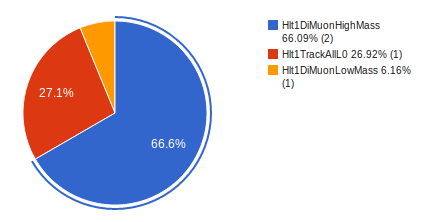
\includegraphics[width=100mm]{profiler/fig12.png}
\caption{\label{fig12}CPU Time percentage of top-level algorithms in the \gaudi sequence tree.}
\end{center}
\end{minipage}
\end{figure}

The report on Figure~\ref{fig12} was produced by a user application that took
an exported  comma-separated-values (CSV) data and compiled it to javascript
code that can be inserted to any dynamic web page.

\section{Results}
In this chapter we presented the \gaudi Intel Performance Auditor --- a CPU
profiling tool that is used in \lhcb experiment at CERN. This tool integrates
the functionality of \iamp performance profiler to the \lhcb core framework
\gaudi. The key advantage of the auditor is an ability to produce reports that
use the framework's modules to present performance analysis results. Those
reports help  developers to identify hotspots in the code and improve the
application performance. Besides the reports, the \gaudi Intel Performance
Auditor provides the options that allow to control the \iamp supervisor's
process from the \gaudi applications.

The results have further strengthened our confidence in the profiling sampling
technique. This technique gives us a reasonable overhead of total profiling
time (5\% at \iamp) in comparison to the tools that count the functions calls.
For example, the popular profiling tool Valgrind~\cite{valgrind} counts every
code instruction and programs running under this tool usually run from five to
twenty times  slower than running outside Valgrind. Though Valgrind provides
precise measurements, using the sampling technique we can get accurate results
by tuning the sampling interval or increasing the number of processing events.

Software optimization has received much attention in the last two years at
\lhcb. To obtain precise information of the general performance, to make
profiling results comparable and to verify the influences of improvements in
the framework or of specific algorithms, it is important to rely on
standardized profiling and regression tests. Software metrics can be created
from the profiling results to monitor the changes in performance and to create
reports on a regular basis if modifications lead to significant
performance degradations. Therefore, for this purpose a system for systematic
profiling is developing at \lhcb, where the \gaudi Intel Profiling Auditor
is one of the main parts.
% \section{Introduction}
% \section{Overview}
% \section{Gaudi Intel Profiler Auditor}
% \section{High Level Trigger profiling}
% \section{Results}
% \section{Conclusions}

\chapter{Study of $\chi_{b}$ production}
\section{Introduction}
\section{Datasets used}
\subsection{Data}
\subsection{Simulated event samples}
\section{$\Upsilon$ selection}
\section{$\chi_{b} \rightarrow \Upsilon \gamma$ selection}
\subsection{Fitting}
\subsection{Optimization}
\subsection{Number of $\chi_{b}$ candidates as function of $p_{T} (\Upsilon)$}

\section{Measurement of $\chi_{b} (3P)$ mass}

\chapter{Systematic uncertainties}
\chapter{Conclusions}

\section*{Acknowledgements}

\renewcommand{\bibname}{References}%  Change the section name from "Bibliography" to "References"

\setboolean{inbibliography}{true}
\bibliographystyle{bib/LHCb}
\bibliography{bib/main,bib/perf,bib/LHCb-PAPER,bib/LHCb-CONF,bib/LHCb-DP}
\end{document}


